% Options for packages loaded elsewhere
\PassOptionsToPackage{unicode}{hyperref}
\PassOptionsToPackage{hyphens}{url}
%
\documentclass[
]{article}
\usepackage{amsmath,amssymb}
\usepackage{lmodern}
\usepackage{ifxetex,ifluatex}
\ifnum 0\ifxetex 1\fi\ifluatex 1\fi=0 % if pdftex
  \usepackage[T1]{fontenc}
  \usepackage[utf8]{inputenc}
  \usepackage{textcomp} % provide euro and other symbols
\else % if luatex or xetex
  \usepackage{unicode-math}
  \defaultfontfeatures{Scale=MatchLowercase}
  \defaultfontfeatures[\rmfamily]{Ligatures=TeX,Scale=1}
\fi
% Use upquote if available, for straight quotes in verbatim environments
\IfFileExists{upquote.sty}{\usepackage{upquote}}{}
\IfFileExists{microtype.sty}{% use microtype if available
  \usepackage[]{microtype}
  \UseMicrotypeSet[protrusion]{basicmath} % disable protrusion for tt fonts
}{}
\makeatletter
\@ifundefined{KOMAClassName}{% if non-KOMA class
  \IfFileExists{parskip.sty}{%
    \usepackage{parskip}
  }{% else
    \setlength{\parindent}{0pt}
    \setlength{\parskip}{6pt plus 2pt minus 1pt}}
}{% if KOMA class
  \KOMAoptions{parskip=half}}
\makeatother
\usepackage{xcolor}
\IfFileExists{xurl.sty}{\usepackage{xurl}}{} % add URL line breaks if available
\IfFileExists{bookmark.sty}{\usepackage{bookmark}}{\usepackage{hyperref}}
\hypersetup{
  pdftitle={Validating morphological condition indices and their relationship with reproductive success in great-tailed grackles},
  pdfauthor={Berens JM1; Folsom M2; Sevchik A1; Bergeron L3; Logan CJ2; McCune KB3*},
  hidelinks,
  pdfcreator={LaTeX via pandoc}}
\urlstyle{same} % disable monospaced font for URLs
\usepackage[margin=1in]{geometry}
\usepackage{graphicx}
\makeatletter
\def\maxwidth{\ifdim\Gin@nat@width>\linewidth\linewidth\else\Gin@nat@width\fi}
\def\maxheight{\ifdim\Gin@nat@height>\textheight\textheight\else\Gin@nat@height\fi}
\makeatother
% Scale images if necessary, so that they will not overflow the page
% margins by default, and it is still possible to overwrite the defaults
% using explicit options in \includegraphics[width, height, ...]{}
\setkeys{Gin}{width=\maxwidth,height=\maxheight,keepaspectratio}
% Set default figure placement to htbp
\makeatletter
\def\fps@figure{htbp}
\makeatother
\setlength{\emergencystretch}{3em} % prevent overfull lines
\providecommand{\tightlist}{%
  \setlength{\itemsep}{0pt}\setlength{\parskip}{0pt}}
\setcounter{secnumdepth}{-\maxdimen} % remove section numbering
\usepackage[left]{lineno}
\linenumbers
\usepackage{booktabs}
\usepackage{longtable}
\usepackage{array}
\usepackage{multirow}
\usepackage{wrapfig}
\usepackage{float}
\usepackage{colortbl}
\usepackage{pdflscape}
\usepackage{tabu}
\usepackage{threeparttable}
\usepackage{threeparttablex}
\usepackage[normalem]{ulem}
\usepackage{makecell}
\usepackage{xcolor}
\ifluatex
  \usepackage{selnolig}  % disable illegal ligatures
\fi
\newlength{\cslhangindent}
\setlength{\cslhangindent}{1.5em}
\newlength{\csllabelwidth}
\setlength{\csllabelwidth}{3em}
\newenvironment{CSLReferences}[2] % #1 hanging-ident, #2 entry spacing
 {% don't indent paragraphs
  \setlength{\parindent}{0pt}
  % turn on hanging indent if param 1 is 1
  \ifodd #1 \everypar{\setlength{\hangindent}{\cslhangindent}}\ignorespaces\fi
  % set entry spacing
  \ifnum #2 > 0
  \setlength{\parskip}{#2\baselineskip}
  \fi
 }%
 {}
\usepackage{calc}
\newcommand{\CSLBlock}[1]{#1\hfill\break}
\newcommand{\CSLLeftMargin}[1]{\parbox[t]{\csllabelwidth}{#1}}
\newcommand{\CSLRightInline}[1]{\parbox[t]{\linewidth - \csllabelwidth}{#1}\break}
\newcommand{\CSLIndent}[1]{\hspace{\cslhangindent}#1}

\title{Validating morphological condition indices and their relationship
with reproductive success in great-tailed grackles}
\author{Berens JM\textsuperscript{1} \and Folsom
M\textsuperscript{2} \and Sevchik A\textsuperscript{1} \and Bergeron
L\textsuperscript{3} \and \href{http://CorinaLogan.com}{Logan
CJ}\textsuperscript{2} \and \href{https://www.kelseymccune.com/}{McCune
KB}\textsuperscript{3}*}
\date{2021-07-25}

\begin{document}
\maketitle

\hypertarget{affiliations}{%
\subparagraph{Affiliations:}\label{affiliations}}

\begin{enumerate}
\def\labelenumi{\arabic{enumi})}
\tightlist
\item
  Arizona State University School of Life Sciences
\item
  Max Planck Institute for Evolutionary Anthropology
\item
  University of California Santa Barbara
\end{enumerate}

*Corresponding author: KB McCune
(\href{mailto:kelseybmccune@gmail.com}{\nolinkurl{kelseybmccune@gmail.com}})

\textbf{Cite as:} Berens JM, Logan CJ, Folsom M, Sevchik A, Bergeron L,
McCune KB. Submitted to PCI Ecology Nov 2020.
\href{http://corinalogan.com/Preregistrations/gcondition.html}{Validating
morphological condition indices and their relationship with reproductive
success in great-tailed grackles}.

\textbf{This preregistration has been pre-study peer reviewed and
received an In Principle Acceptance by:}

Marcos Mendez (2019 In Principle Acceptance) Are condition indices
positively related to each other and to fitness?: a test with grackles.
\emph{Peer Community in Ecology}, 100035.
\href{https://doi.org/10.24072/pci.ecology.100035}{10.24072/pci.ecology.100035}

\begin{itemize}
\tightlist
\item
  Reviewers: Javier Seoane and Isabel López-Rull
\end{itemize}

\hypertarget{abstract}{%
\section{ABSTRACT}\label{abstract}}

Morphological and physiological variation among individuals has the
potential to influence multiple life history characteristics such as
dispersal, migration, reproductive success, and survival. Individuals
that are in better ``condition'' can disperse or migrate further or more
successfully, have greater reproductive success, and survive longer,
particularly in years where environmental conditions are harsh.
Condition is defined in various ways, but is most often measured using
an individual's energetic state. These traits are difficult to measure
directly, therefore a variety of morphological proxies to quantify
energetic condition are used instead, including fat score, weight, ratio
of weight to tarsus length, and a scaled mass index. However, there is
mixed support regarding whether these energetic condition indices relate
to life history characteristics, and whether the relationship is linear.
Additionally, although some investigations use multiple morphological
proxies for energetic condition, rarely have there been direct
comparisons among proxies to validate that they measure the same trait.
In this investigation, we define condition as an energetic state and we
attempt to measure it by comparing two morphological indices (fat score
and the scaled mass index) to validate whether they measure the same
trait and whether they correlate with measures of reproductive success
in our study system, the great-tailed grackle (\emph{Quiscalus
mexicanus}). We found that the morphological proxies did not correlate
with each other, indicating that they do not measure the same trait.
Further, neither proxy significantly correlated with reproductive
success in males, measured as whether a male held a territory containing
nests or not. We found that females with a high scaled mass index had a
significantly lower probability that their nest would survive on any
given day. However, there was no relationship between female fat score
and nest survival. These results indicate that morphological measures of
energetic condition should be validated before relying on their use as a
condition proxy in grackles and birds in general. Future research should
investigate behavioral mechanisms underlying our result that higher
scaled mass index correlated with lower nest survival to better
understand the importance of energetic condition for reproductive
success - a necessary component for selection to act.

\hypertarget{introduction}{%
\section{INTRODUCTION}\label{introduction}}

Morphological and physiological variation among individuals has the
potential to influence multiple life history characteristics such as
dispersal, migration, reproductive fitness, and survival (Wilder et al.,
2016). One trait that might be particularly likely to influence these
life history characteristics is energetic condition. Individuals that
are in better ``condition'' can disperse or migrate further or more
successfully, have greater reproductive success, and survive longer
(Heidinger et al., 2010; Liao et al., 2011; Wilder et al., 2016),
particularly in years where environmental conditions are harsh
(Milenkaya et al., 2015). For example, a study conducted on vipers
showed that while the level of fat reserves in males was not related to
their sexual activity, females with low fat reserves engaged in sexual
interactions less frequently than those with higher fat reserves (Aubret
et al., 2002). In contrast, mantids showed conflicting results regarding
the relationship between fat reserves and reproductive success (Barry \&
Wilder, 2013). Female mantids were fed either a high protein, low lipid
diet, or a high lipid, low protein diet. The females that received the
high lipid diet had higher lipid content in most parts of their body
compared to that of their high protein diet counterparts. However, they
were not able to produce even half as many eggs as the females fed the
high protein, low lipid diet. This led to lower male attraction,
measured by the number of copulation events, thus negatively impacting
further reproductive success.

A variety of morphological proxies have been used to quantify energetic
condition {[}i.e., fat score, weight, ratio of mass to structural size,
residuals from a linear regression of mass as a function of structural
body size; Labocha et al. (2014); Jacobs et al. (2012){]}. However,
there is mixed support regarding whether and how these proxies relate to
life history characteristics (Labocha et al., 2014; Wilder et al.,
2016). A review conducted by Barnett (2015) shows that, while mass or
body size measures of energetic condition are often assumed to have a
positive linear relationship with fitness, this is not always the case,
and the relationship should first be empirically validated before being
used as a proxy (Barnett et al., 2015). In some instances, the proxy
might relate to life history characteristics, but in a non-linear way.
For example, theoretical simulations of small birds show that survival
does not increase linearly with energy (i.e., fat) reserves (McNamara et
al., 2005). If the reserves are too low, the individual is at risk of
starvation. However, once the reserves get too high, the individual is
at an increased risk of predation (McNamara et al., 2005). Thus, fat
reserves can relate to a life history variable (survival), but in a
U-shaped relationship rather than a linear one.

Although some studies use multiple morphological proxies for energetic
condition (e.g., Warnock \& Bishop, 1998), rarely are these variables
directly compared. Multiple proxies should correlate with each other if
they measure the same trait (energetic condition). Furthermore, there is
still confusion about what trait some proxies actually measure. For
example, a study conducted on two species of crickets showed that three
estimates of energetic condition based on fat content or on the
relationship between body mass and body length (scaled mass index or
ordinary least squares regression) did not correlate with each other
(Kelly et al., 2014). A similar lack of a relationship was found in
flying animals such as birds (A. G. Gosler et al., 1995; Jacobs et al.,
2012) and bats (McGuire et al., 2018) thus indicating cross-taxa support
that morphological proxy measures do not always measure the same trait.
This is an example of the jingle fallacy (Block, 1995; Carter et al.,
2013), where a single trait label (``energetic condition'') actually
encompasses more than one distinct trait. In this case, two
investigations using different proxies can be conducted on the same
research question, using the same species, but may end up with different
results. This is problematic because inconsistency in results among
researchers can result in potentially misleading interpretations of the
impact of variation in morphology in relation to life history and
population variables (Stevenson \& Woods Jr, 2006).

Here we compare two indices (fat score and the scaled mass index) of an
individual's energetic state to validate whether they correlate with
each other, which would indicate that they both measure energetic
condition. Fat score, as described by Kaiser (1993), is a numerical
estimate of the amount of fat visible under the skin (Fig. 1). The score
ranges from 0 to 8 depending on the size and appearance of the fat
located in the individual's abdomen and interclavicular depression, with
0 indicating no visible fat and 8 indicating extensive fat covering the
ventral surface such that no muscle tissue is visible. For example, a
score of 1 corresponds to sparse traces of fat visible in the
interclavicular depression and abdomen. This measure is frequently used
in birds (Cornelius Ruhs et al., 2019; Erciyas et al., 2010; Merilä \&
Svensson, 1997), and is a straightforward, non-invasive method for
estimating energetic condition. However, previous research found that it
does not always positively relate with life history variables. For
example, Haas (1998) found no difference between fat scores in
individuals that had successful or failed nests in American robins and
brown thrashers, indicating that fat score may not explain much of the
variation in nest success in some species. Further research is needed to
understand the relationship between fat score measures and life history
characteristics.

In contrast, the scaled mass index (SMI) is more difficult to calculate
than the fat score, but it has become the predominant ratio method for
quantifying energetic condition within and among populations (Delciellos
et al., 2018; English et al., 2018; Maceda-Veiga et al., 2014). The SMI
is an individual's mass scaled by skeletal body size (Peig \& Green,
2009). Unlike the common alternative which uses a simple ratio of tarsus
(lower leg) length to body mass, the SMI accounts for the tendency
towards allometric scaling where the relationship between body mass and
structural size increases by a power law (Huxley, 1932). When
individuals with different structural body sizes can be standardized to
the population average structural body size, then energetic condition
(the amount of mass not explained by structural body size) can be more
directly compared within and across populations. That is, the SMI
calculates the energetic condition as the mass of an individual relative
to the population by first computing the mass that the individual would
have at the population average of a specific body measurement (e.g.,
tarsus length). Next, structural body size of the individual is
standardized by scaling the individual's structural body length by the
population average of that body measurement, which accounts for
population differences. The SMI is calculated as:
\(Mass_i\left[ \frac{AvgLength_p}{Length_i} \right]^{slope_p}\) where
\(Mass_i\) is each individual's weight in grams, \(Length_i\) is the
value of the chosen measure of structural body length for each bird,
\(AvgLength_p\) is the average structural body length in the population,
and \(slope_p\) is calculated from the standard major axis regression
(which is used to compare variables that were both directly measured and
thus have residual error) of a structural body size measure, like tarsus
length on mass (Peig \& Green, 2009), and is interpreted as the expected
change in structural length for a one unit increase in mass. Therefore,
individuals with superior energetic condition (larger weight for their
structural body size) will have a higher SMI compared to individuals
that with inferior energetic condition. Studies across taxa found that
the SMI relates positively to reproductive success and survival. For
example, mallards with a lower SMI had lower rates of survival compared
to their higher SMI counterparts (Champagnon et al., 2012), while in
crimson finches SMI was positively related to the number of young that
survived to independence (Milenkaya et al., 2015).

Our research will determine whether these two indices of energetic
condition measure the same trait, and whether this trait relates to an
important life history characteristic: reproductive success. Measuring
reproductive success in birds involves finding and monitoring nests
(Mayfield, 1961). However, nests are usually built in cryptic locations
and parents behave secretly (Gill, 1995), thus making it difficult to
quantify the number of eggs and nestlings inside the nest over time.
Additionally, it is difficult and time-consuming to track the survival
of offspring once they leave the nest. Therefore, we will use the
predominant method in this field for quantifying reproductive success:
whether a nest fledged offspring (Mayfield, 1961).

Our study system is a population of great-tailed grackles
(\emph{Quiscalus mexicanus}), hereafter ``grackles,'' in Tempe, Arizona.
This system is ideal for this investigation because grackles are native
to the tropical climates of Central America (Johnson \& Peer, 2001), but
have rapidly expanded their geographic range into new areas (Wehtje,
2003). Because grackles are a water-associated species, the desert
habitat of Tempe presents physiological challenges that could lead to an
increased likelihood of a tradeoff between survival and reproductive
attempts (Henderson et al., 2017). Deserts are characterized by a
scarcity of water and extreme temperature fluctuations, which require
behavioral and physiological adaptations (Costa, 2012). Wide variation
in energetic condition and reproductive success is possible if grackle
physiology requires more water than is present in the environment, and
some individuals may cope with physiological stress, or find hidden
sources of water, better than others (Henderson et al., 2017).

\hypertarget{hypotheses}{%
\paragraph{\texorpdfstring{\textbf{Hypotheses}}{Hypotheses}}\label{hypotheses}}

We measured two morphological proxy variables of energetic condition and
observed reproductive success in grackles to test two hypotheses. The
first examined the relationship between two morphological proxies of
energetic condition to validate that they measure the same inherent
trait. Secondly, we hypothesized that energetic condition, as measured
by either or both of the morphological proxy variables, would relate to
reproductive success in male and female grackles.

\hypertarget{methods}{%
\section{METHODS}\label{methods}}

The methods below are based on the preregistration, with small changes
summarized in the Deviations from the planned methods section and
further explained in the preregistration (in italics).

\hypertarget{preregistration-details}{%
\paragraph{\texorpdfstring{\textbf{Preregistration
details}}{Preregistration details}}\label{preregistration-details}}

The preregistration used secondary data that were collected as part of
other ongoing investigations (tarsus length in
\url{http://corinalogan.com/Preregistrations/g_flexgenes.html}; tarsus
length, body weight, number of fledglings, and whether a male holds a
territory in
\url{http://corinalogan.com/Preregistrations/g_withinpop.html}; and
tarsus length in
\url{http://corinalogan.com/Preregistrations/g_expansion.html}). The
preregistration, containing the hypotheses, methods, and analysis plan,
was written (July 2019) and submitted to Peer Community In Ecology for
pre-study peer review (August 2019) before any analyses were conducted.
We revised according to reviewer comments and received in principle
acceptance by PCI Ecology of the version on 8 Nov 2019. After that, we
conducted the analyses in the preregistration. Our final methods,
results, and discussion, including all data and code, are listed below.

\hypertarget{summary-of-methods}{%
\paragraph{\texorpdfstring{\textbf{Summary of
methods}}{Summary of methods}}\label{summary-of-methods}}

Great-tailed grackles are caught year-round in the wild in Tempe,
Arizona using a variety of methods (e.g., walk-in trap, bownet, mist
net). After capture we immediately processed birds by attaching colored
leg bands in unique combinations for individual identification,
conducted morphological measurements of weight, tarsus length, flattened
wing length, tail length, skull length, bill length and fat score (Fig.
1, the amount of visible fat under the skin in the clavicle and abdomen
as in Kaiser, 1993). Most grackles were released after completion of
color band marking, measurements, and acquiring a blood sample. A subset
of grackles were held in aviaries for up to 6 months for behavioral
testing, and then released back to the wild at their location of
capture. We tested the repeatability of our structural size measures on
this subset of individuals by measuring them again before release. The
second measures were collected by the same experimenter in 11 out of 17
females and 10 out of the 18 males that were repeatedly sampled.

\includegraphics[width=0.25\textwidth,height=\textheight]{gconditionfig1a.jpg}
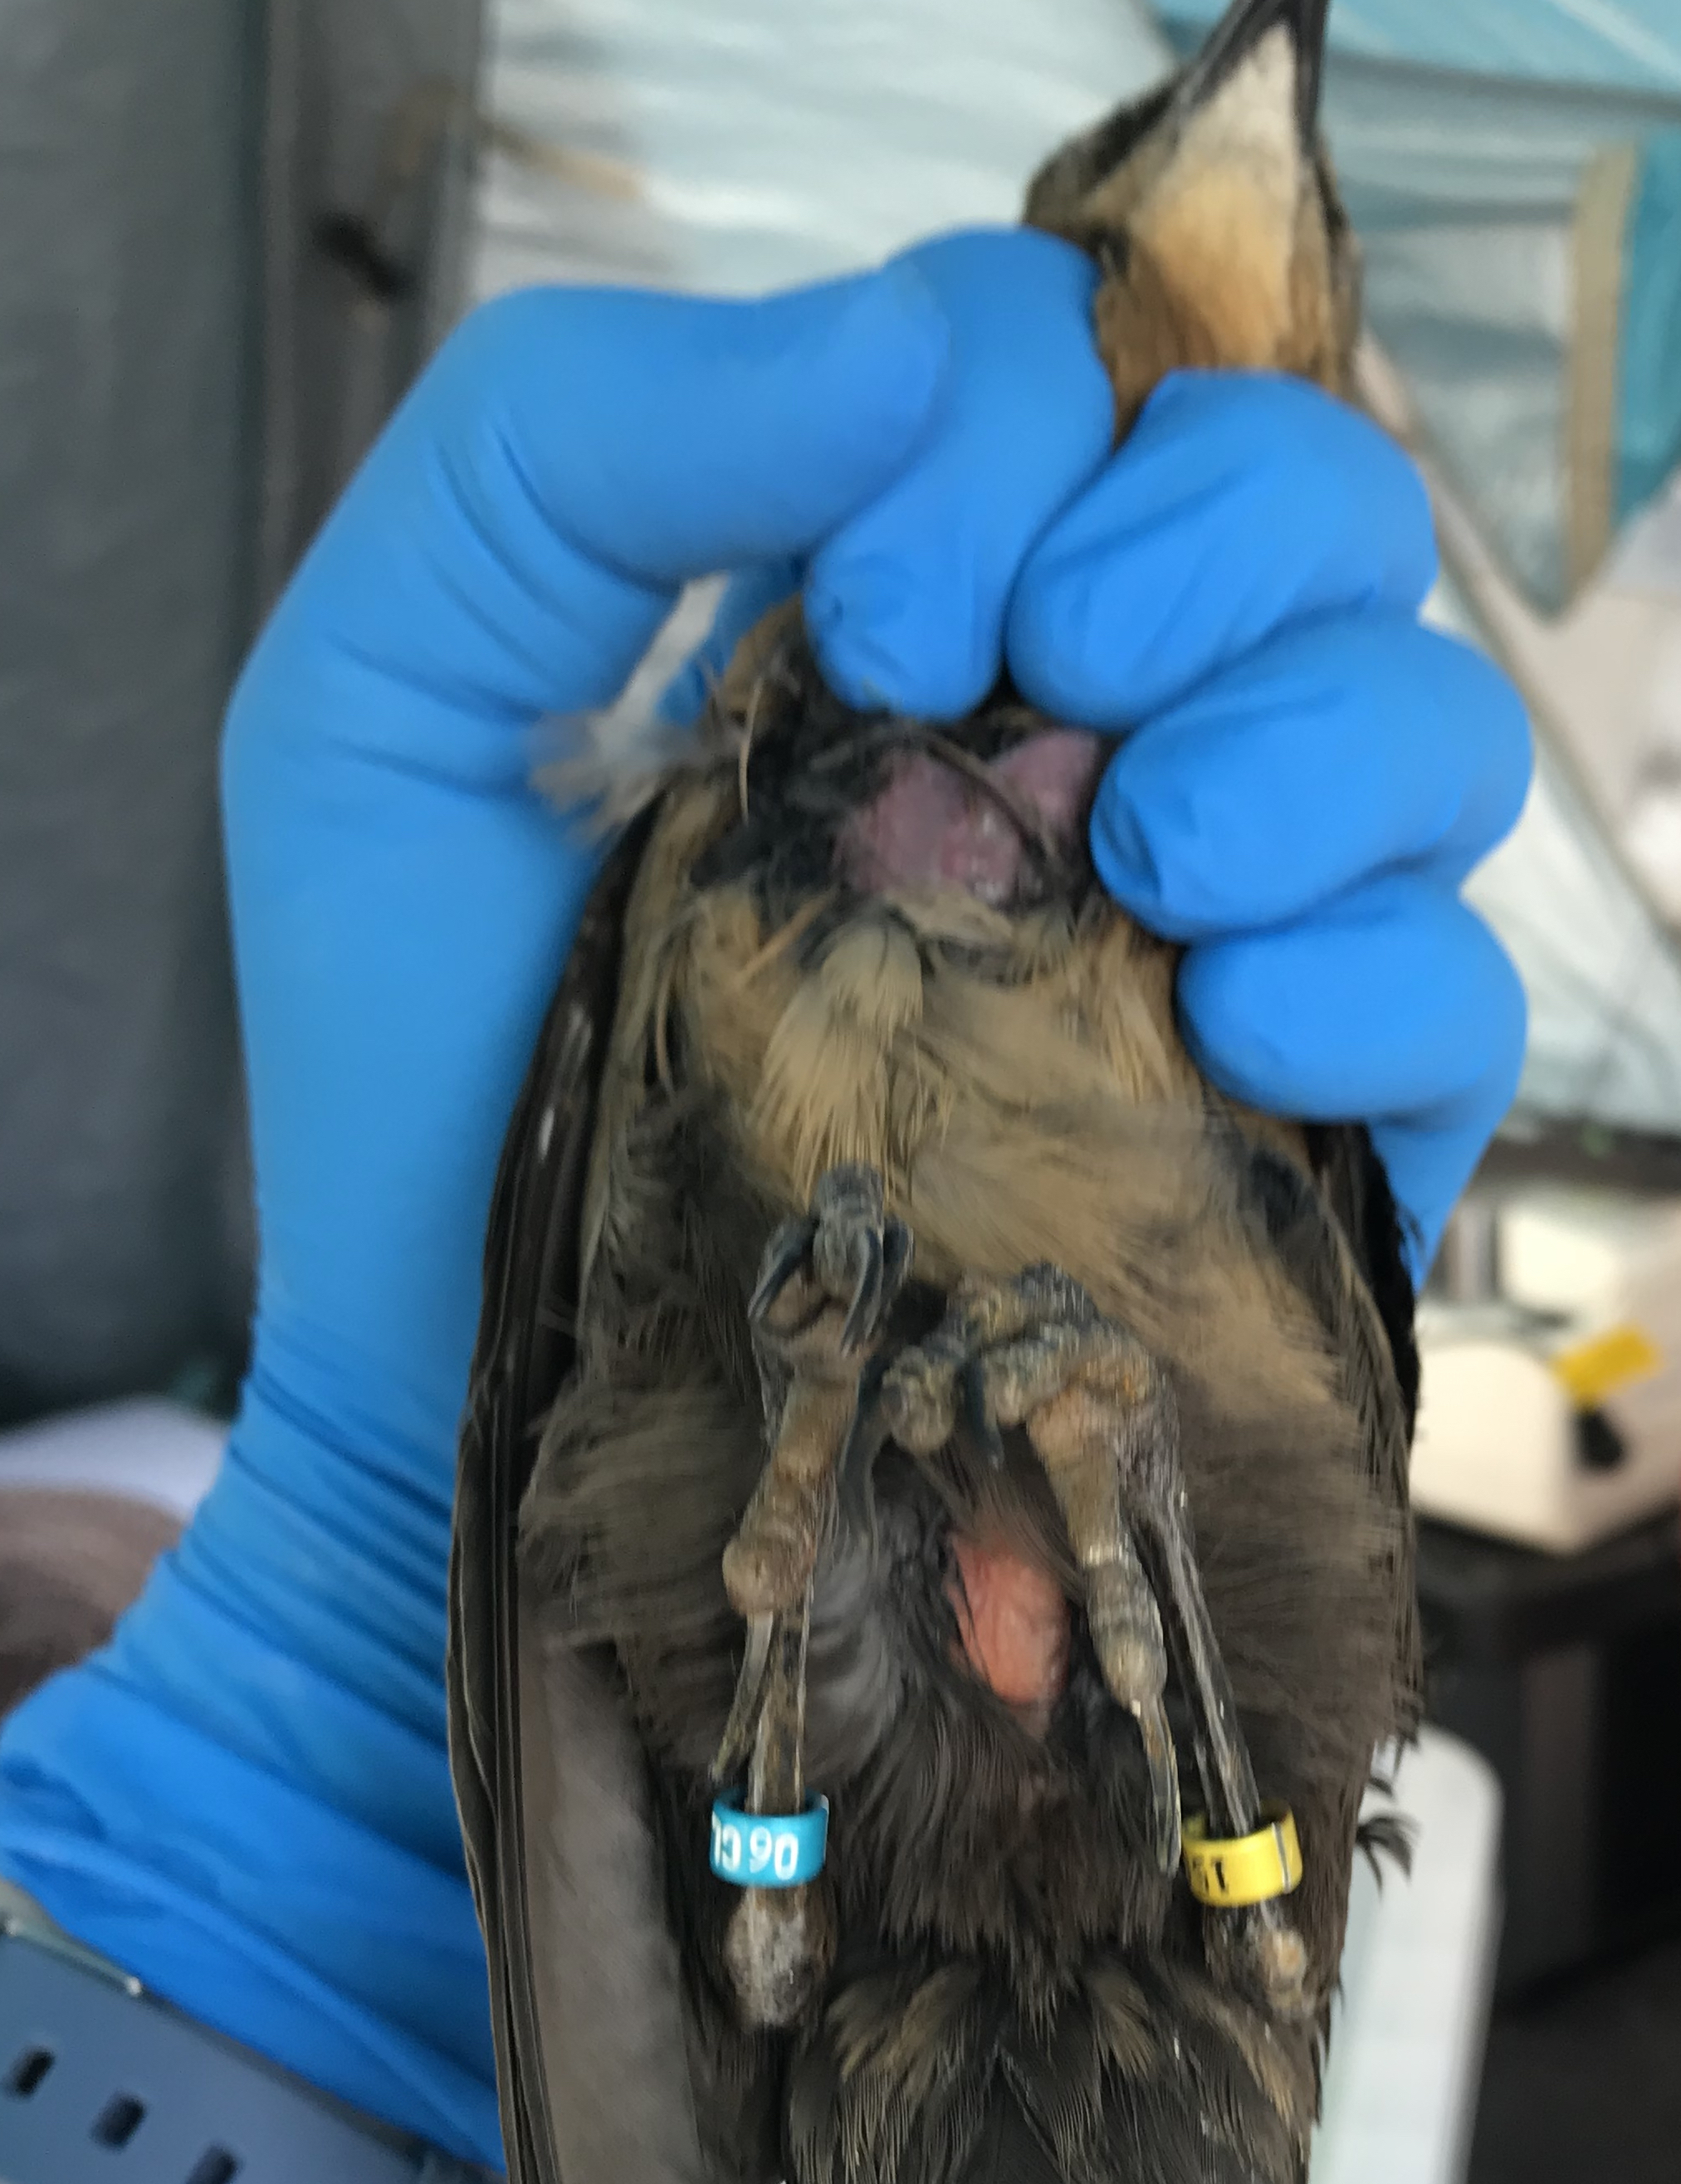
\includegraphics[width=0.25\textwidth,height=\textheight]{gconditionfig1b.jpg}

Figure 1: A male grackle showing the yellow/orange tint of fat under the
skin in the intraclavicular depression (left); and a female grackle
showing \emph{no} fat under the skin of the intraclavicular region, but
significant fat deposits under the skin of the abdomen (right).

From March - August, we monitor the behavior of all color-marked
grackles to determine their nesting status. We follow females carrying
nesting materials to find their nest. We determine whether the male
territory owner is color-marked as well. Then we check each nest
approximately every day to determine the status based on the female's
behavior (building, incubation, feeding nestlings, feeding fledglings,
failed).

Individuals included in our sample were those for which we have measures
of energetic condition when they were adults. We did not include
individuals whose data were collected as juveniles. We also excluded
data that was collected from the grackles when they were released from
the aviaries to avoid any confounds due to their time in the aviary
(e.g., perhaps unlimited nutritious food in the aviaries affected their
fat score). However, to validate that our measures of structural body
size (tarsus length or wing length) are precise and accurate, we
measured twice the subset of grackles brought into aviaries - once when
they were initially caught, and again up to 6 months later when we
released them. We calculated the repeatability of these multiple
measures. All other data included in this study came from wild-caught
grackles (including the data from the birds that were brought into the
aviaries on their first capture).

We first used logistic mixed-effect models to determine whether SMI and
fat score are correlated. We also tested whether SMI and fat score
varied by season because grackles are difficult to catch such that we
were unable to structure our data collection to coincide with the
breeding season and instead caught and measured grackles as often as
possible. Previous research found a non-linear relationship between
reproductive success and energetic condition variables (Milenkaya et
al., 2015). To check whether this is occurring in our data, we visually
examined our raw data to determine if we need to include a non-linear
energetic condition independent variable into our models
(i.e.~FatScore\textsuperscript{2}). Then we used we used two types of
logistic mixed-effect models to determine the relationship between
energetic condition and reproductive success. Both types are supported
in the literature, but are slightly different in the way in which the
link function is specified. First, we modeled the effect of energetic
condition on reproductive success using a generalized linear mixed model
framework with a logit link function (i.e. Milenkaya et al., 2015). We
then also used a logistic exposure model that has a link function which
accounts for the time interval between nest checks when estimating the
probability of daily nest survival (Bolker, 2014; Shaffer, 2004).

\hypertarget{after-pre-study-peer-review-deviations-from-the-planned-methods}{%
\paragraph{\texorpdfstring{\textbf{After pre-study peer review:
Deviations from the planned
methods}}{After pre-study peer review: Deviations from the planned methods}}\label{after-pre-study-peer-review-deviations-from-the-planned-methods}}

\begin{enumerate}
\def\labelenumi{\arabic{enumi})}
\item
  We realized that the sexual dimorphism of male and female body sizes
  necessitates separate analyses. Therefore, we calculated SMI for males
  and females separately, and ran separate models for each sex for the
  repeatibility analysis (P1 and P2).
\item
  Fat score data were distributed such that the majority of scores were
  0, with some 1's and very few higher numbers. Specifically, of the 21
  males, 15 had fat scores at 0, 5 scored 1, and a single male had a fat
  score of 2. Out of 47 females, 26 scored 0, 18 scored 1, 2 scored 2,
  and a single female scored 3. This lack of variance in the response
  variable led to problems when we ran the models: it was difficult to
  fit models using an ordinal regression. The function
  ``simulateResiduals,'' which we used to check our data, does not work
  with data in the ordinal family. Consequently, we modified the model
  to use a logistic regression where the dependent variable FatScore is
  categorized as individuals that showed no visible fat (y = 0), or some
  fat was present (y = 1) where we combined all individuals that had fat
  score values of 1 or greater. Subsequent data checking indicated that
  these data were not zero-inflated or overdispersed.
\end{enumerate}

\hypertarget{deviations-when-testing-hypothesis-1-correlation-between-smi-and-fat-score}{%
\subparagraph{Deviations when testing hypothesis 1: correlation between
SMI and Fat
score}\label{deviations-when-testing-hypothesis-1-correlation-between-smi-and-fat-score}}

\begin{enumerate}
\def\labelenumi{\arabic{enumi})}
\setcounter{enumi}{2}
\item
  Warning messages occurred during the repeatability analysis using the
  ``rptR'' package in R (Stoffel et al., 2017) indicating that the fit
  was singular, likely because the variance for the Experimenter random
  effect in the model for both female and male wing length was 0.001. We
  thus conducted an unregistered analysis where we confirmed that our
  repeatability values from the repeatability models were valid, despite
  the warning, by hand calculating repeatability following Nakagawa \&
  Schielzeth (2010). The hand-calculated repeatabilities were nearly
  identical (female R = 0.5, male R = 0.71) to the output from the rpt
  function.
\item
  Despite the data checking which indicated our model was not
  overdispersed or zero inflated, we could not get the fixed effects or
  random effect to converge using the Bayesian package in R
  ``MCMCglmm.'' We found no improvement in model fit by tweaking the
  priors or iterations/burnin/thin options. Therefore, we fit these
  models using the function glmer, a frequentist framework.
\item
  The Season variable only includes 2 males in the breeding season
  category, thus we do not have a large enough sample to produce
  reliable estimates. We removed the Season variable from the model for
  males.
\end{enumerate}

\hypertarget{deviations-when-testing-hypothesis-2-energetic-condition-and-reproductive-success}{%
\subparagraph{Deviations when testing hypothesis 2: energetic condition
and reproductive
success}\label{deviations-when-testing-hypothesis-2-energetic-condition-and-reproductive-success}}

\begin{enumerate}
\def\labelenumi{\arabic{enumi})}
\setcounter{enumi}{5}
\item
  Only two females had reproductive success data from more than one year
  in our study (2019 and 2020). Consequently, there were very few
  repeated measures in this sample and our random effect of bird ID
  accounted for zero variance. This led to a warning that our model fit
  was singular. Therefore, we removed the data for these females for
  2020 so we could remove ID as a random effect from the model, which
  resulted in the model running without warnings. We removed the 2020
  data for these females because their energetic condition data was
  collected in 2019 and these measures were more likely to relate to
  their 2019 reproductive success data than to their reproductive
  success in 2020.
\item
  The fit of the model analyzing the relationship between energetic
  condition and male reproductive success (ability to hold a territory
  containing female nests) was singular. The Year random effect
  accounted for zero variance in the data, so we removed it. The fit was
  still singular, but we retained the ID random effect (although it also
  explained zero variance) to account for repeated measures in this
  sample.
\item
  The model fit was again singular in our logistic exposure model
  because the Year random effect explained zero variance in the data. We
  removed this random effect from the analysis.
\end{enumerate}

\hypertarget{results}{%
\section{RESULTS}\label{results}}

\textbf{Prediction 1: correlation between SMI and Fat Score}

\begin{table}

\caption{\label{tab:sample size table}Table 1. Sample sizes for P1 and P2.  The *Breeding* and *Non-breeding season* categories refer to the number of individuals measured in each season. The *Reprod. success* category represents the total number of individuals in each year observed engaging in breeding behaviors. Note that the 2019 and 2020 reproductive success sample sizes include some of the same individuals that were observed in both years. Whereas, the *Prop. successful* category represents the proportion of the total individuals observed engaging in breeding behaviors in each year that held a territory containing nests (males) or fledged young (females).}
\centering
\begin{tabular}[t]{lcc}
\toprule
Category & Males & Females\\
\midrule
Breeding Season Fat & 2 & 12\\
Non-breeding fat & 20 & 35\\
Breeding season SMI & 6 & 24\\
Non-breeding SMI & 18 & 38\\
Aviaries & 16 & 9\\
\addlinespace
Repro. success 2019 & 8 & 9\\
Repro. success 2020 & 17 & 13\\
Prop. successful 2019 & 0.63 & 0.22\\
Prop. successful 2020 & 0.47 & 0.54\\
\bottomrule
\end{tabular}
\end{table}

\begin{table}

\caption{\label{tab:p1 results}Table 2. Results from the logistic mixed-effect regression for 47 females and fixed-effect regression for 21 males to determine whether fat score and scaled mass index (SMI) are correlated. Estimates are presented with the standard error in parentheses. Our sample size was too small to test for a season effect in males.}
\centering
\begin{tabular}[t]{lcccc}
\toprule
\multicolumn{1}{c}{ } & \multicolumn{2}{c}{Females} & \multicolumn{2}{c}{Males} \\
\cmidrule(l{3pt}r{3pt}){2-3} \cmidrule(l{3pt}r{3pt}){4-5}
Parameter & Estimate (SE) & p-value & Estimate (SE) & p-value\\
\midrule
Intercept & -0.20 (0.74) & 0.79 & -0.82 (0.64) & 0.21\\
SMI & 0.07 (0.30) & 0.81 & 0.46 (0.62) & 0.46\\
Season & 0.27 (0.71) & 0.70 & NA & NA\\
\bottomrule
\end{tabular}
\end{table}

We were able to calculate SMI for 24 males and 62 females, and fat score
values were available for 22 males and 47 females (Table 1).

We found that wing length was more tightly correlated with body mass
than tarsus length in both sexes, therefore we used wing length in our
SMI calculations (female n = 62, r = 0.26, \emph{p} = 0.03; male n = 24,
r = 0.35, \emph{p} = 0.08). This allows us to account for as much
variation in body mass as possible that is associated with skeletal body
size because leftover variation in body mass is more likely to relate to
energetic condition. Consequently, we used wing length in our
calculation of SMI.

To validate that we were measuring structural body size consistently
across experimenters, we analyzed the repeatability of wing length in
the birds in our sample that were measured more than once. We found that
average wing length was repeatable (n = 17 females, Repeatability ±
standard error = 0.53 ± 0.18; n = 18 males, Repeatability ± SE = 0.75 ±
0.11). Data permutations and a likelihood ratio test both confirmed that
these repeatability values were statistically significant at p
\textless{} 0.01.

In females, we found that for every one unit increase in SMI, the bird
is 1.3 times more likely to have some fat (a 30\% increase in the odds
of having fat), which is not a statistically significant relationship
(female \emph{p} = 0.81; Table 2). In males, a one unit increase in SMI
corresponds to an odds ratio of 1.6, or a 60\% increase in the odds of
having some fat, which is also not a statistically significant
relationship (\emph{p} = 0.50; Table 2). Together, this indicates that
SMI and fat score are not equally measuring energetic condition. There
was also no relationship between season (breeding or non-breeding) and
female fat score (\emph{p} = 0.71). Only 2 males were measured during
the breeding season, therefore we omitted season as an independent
variable in the male model (Table 1).

\textbf{Prediction 2: energetic condition and reproductive success}

Our sample size for P2, where individuals had measures of reproductive
success, SMI, and fat scores, was 20 for females and 20 for males.

To determine whether we should include any non-linear effects of SMI in
our models (A. G. Gosler et al., 1995; Milenkaya et al., 2015), we
visually evaluated whether individuals in any of 5 categories, ranging
from low to high SMI, were more likely to be reproductively successful
(Fig. 2). We found no visual evidence for a non-linear relationship
between reproductive success and SMI for males or females (Fig. 3).
Consequently, we did not include non-linear terms in subsequent models.

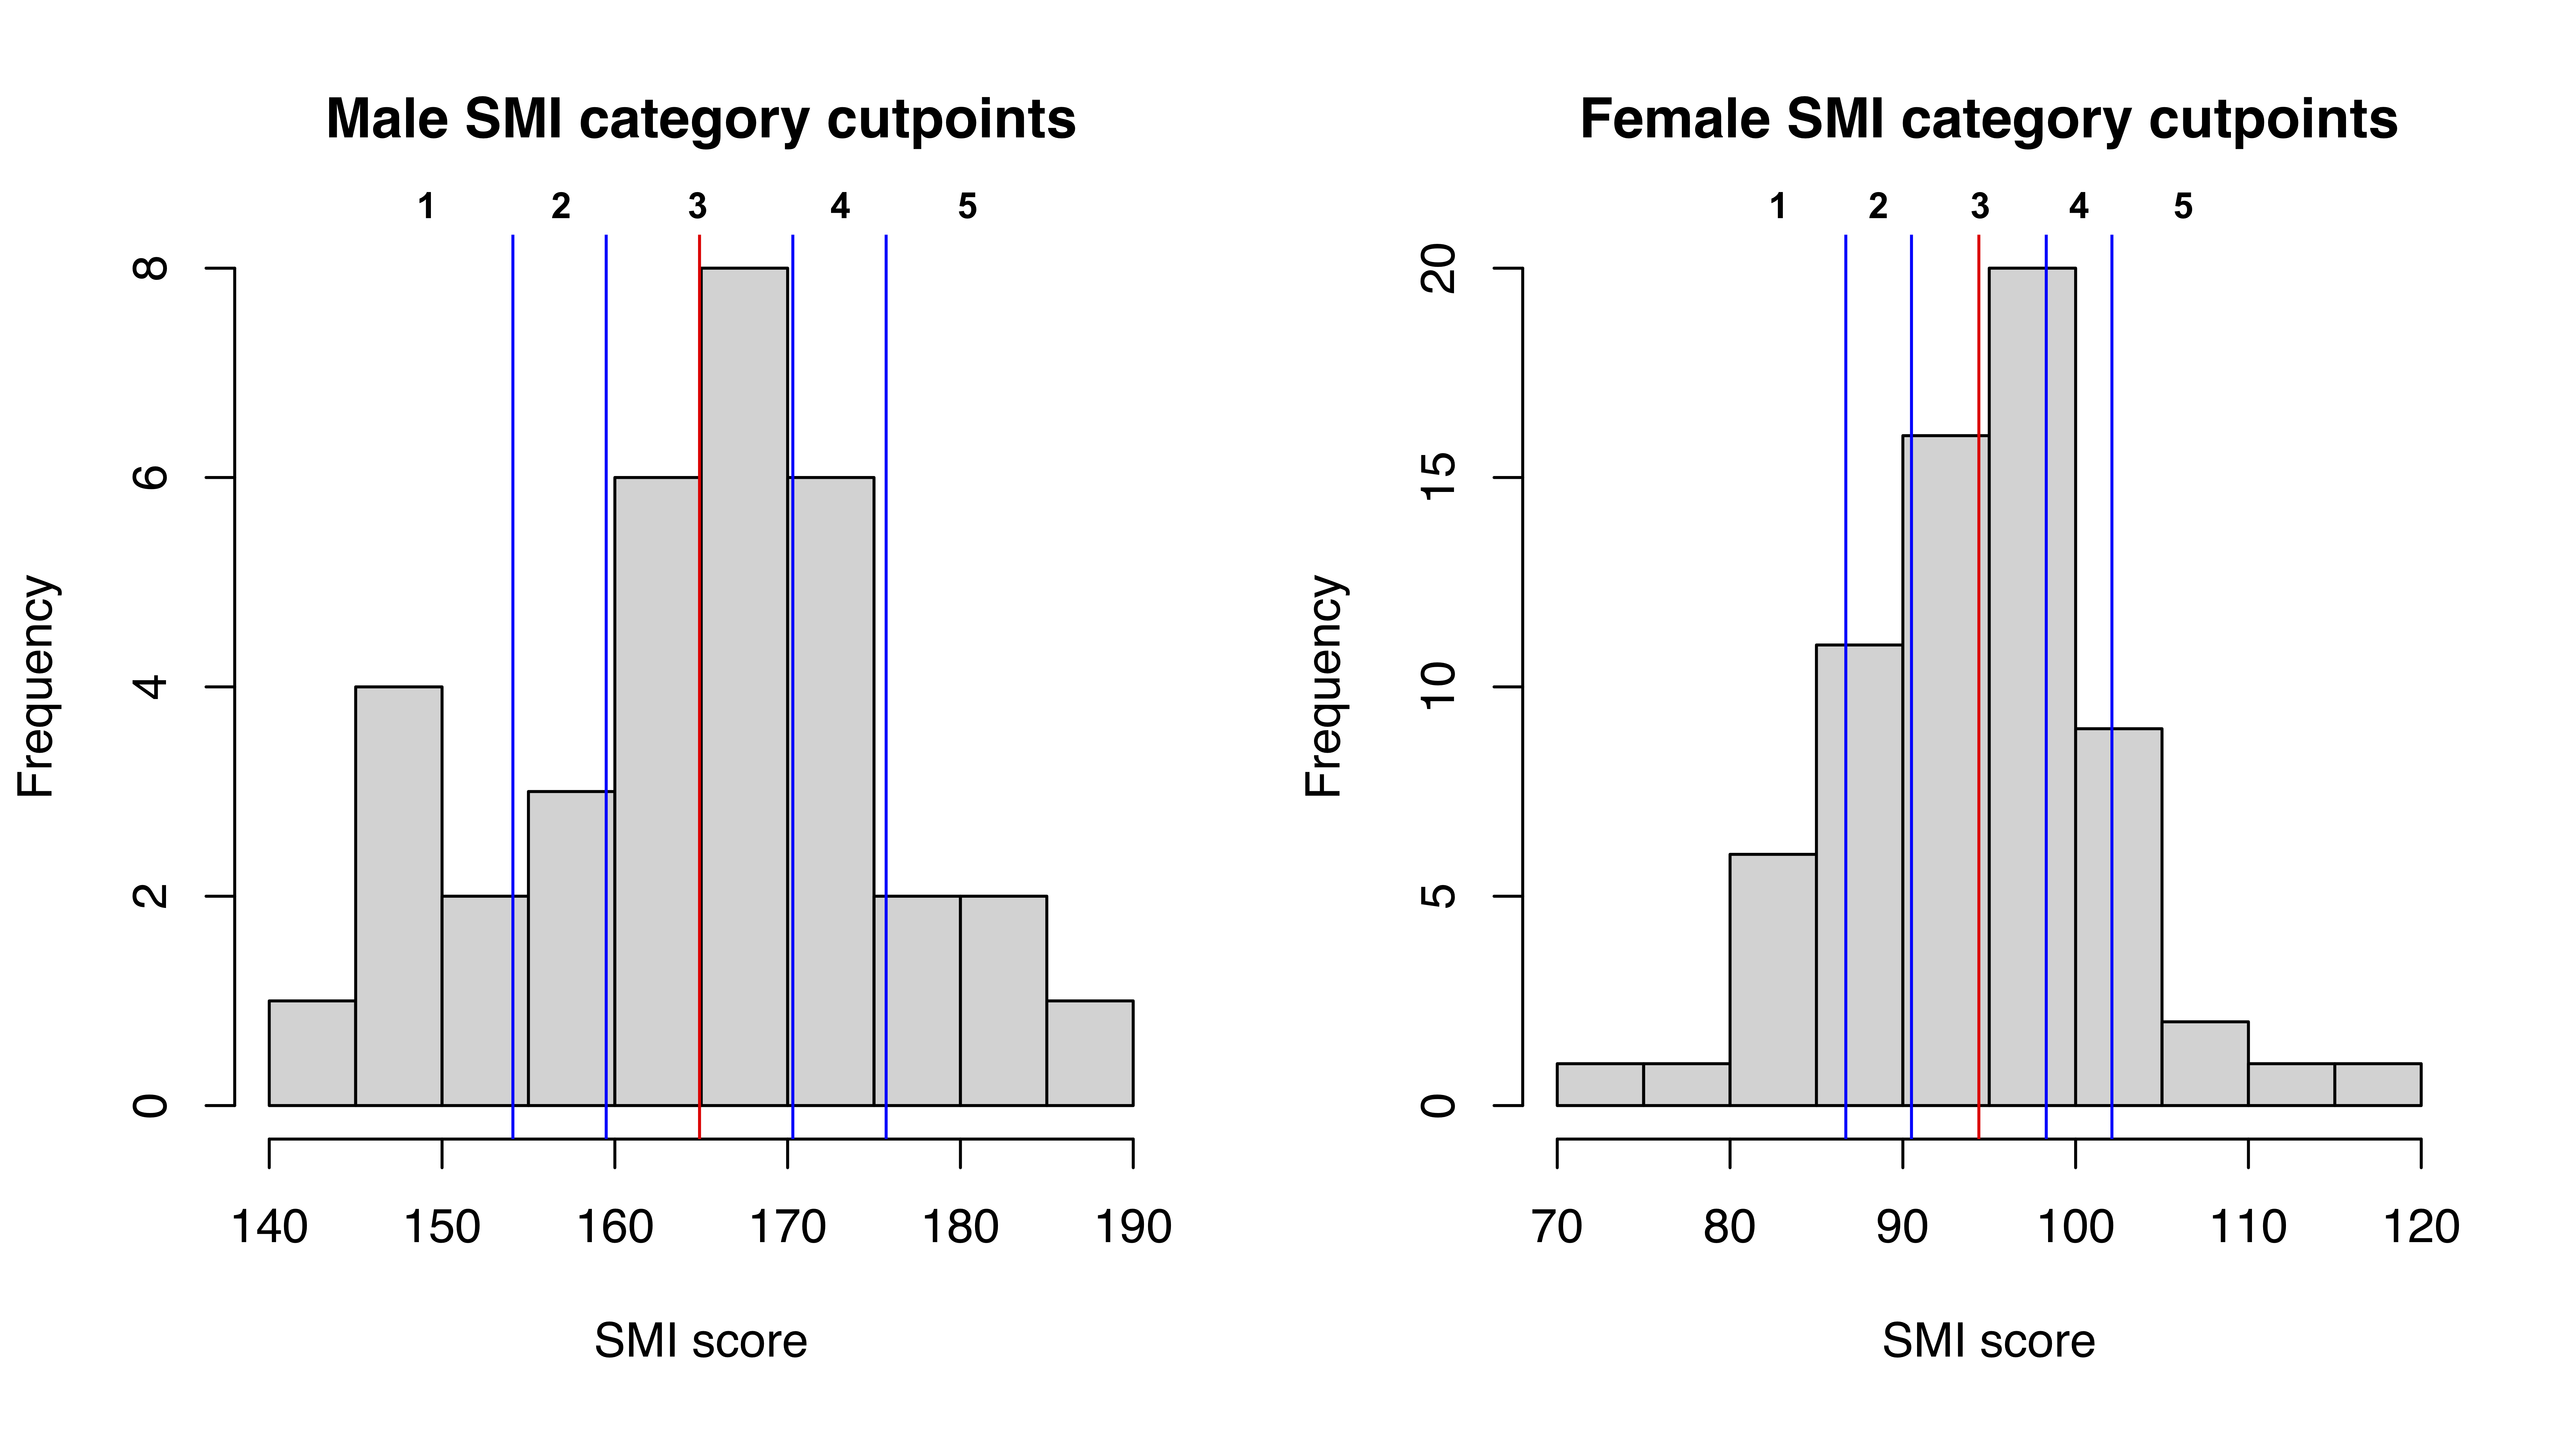
\includegraphics[width=0.85\textwidth,height=\textheight]{gconditionfig2.jpg}

Figure 2: Frequency histogram of the SMI scores, illustrating the SMI
categories, for the 33 males and 31 females for which we also had
reproductive success data. The mean SMI value is indicated by a red
vertical line. We created SMI category bins (indicated with vertical
blue lines) in 1 standard deviation increments, centered on the mean.
Category 3 indicates the SMI value is close to the population mean
value. Categories 1 and 2 are individuals that have SMI scores that are
low, and moderately low, respectively, compared to the population mean
value. Similarly, categories 4 and 5 contain individuals that have SMI
scores that are moderately high and high, respectively, compared to the
population mean value.

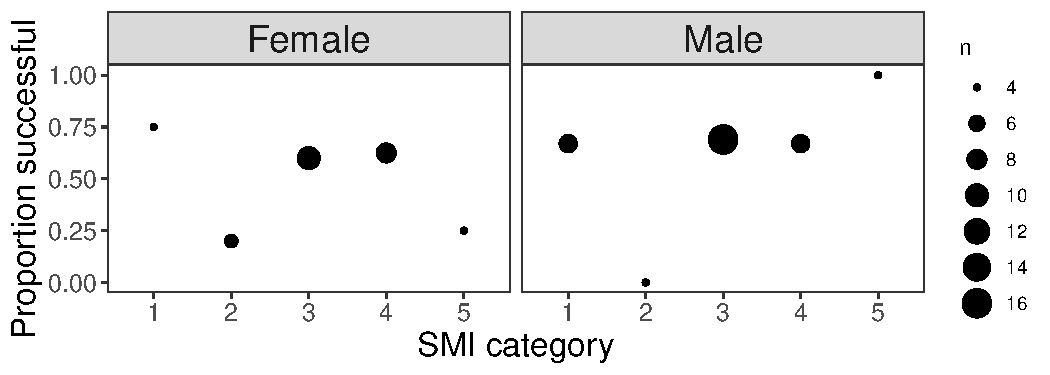
\includegraphics{gcondition_files/figure-latex/p2 non-linear trend results-1.pdf}

Figure 3: The proportion of individuals that successfully fledged nests
(females: left) or held a territory (males: right) in low (1),
moderately low (2), moderate (3), moderately high (4) and high (5)
scaled mass index (SMI) categories. Dots are sized according to the
number (n) of individuals in that category. There is no evidence of a
non-linear relationship.

We used linear models to determine whether season would be important to
include in our models testing whether body condition relates to
reproductive success. We found that SMI did not differ by season for
females (Estimate (SE): \emph{\(\beta\)} = -0.30 (0.26), \emph{p} =
0.26) or males (\emph{\(\beta\)} = -0.65 (0.43),\emph{p} = 0.15).
Similarly, fat score for females (\emph{\(\beta\)} = 0.28 (0.68),
\emph{p} = 0.68) and males (\emph{\(\beta\)} = 17.08 (2797.4), \emph{p}
= 0.99) did not differ by season (Fig. 4). Although we note that, as
stated above and indicated in the standard error value, we lack
sufficient fat score data from males in the breeding season so these
results should be interpreted with caution. Consequently, we did not
include season as an independent variable in our subsequent models
testing the relationship between our body condition proxies and
reproductive success.

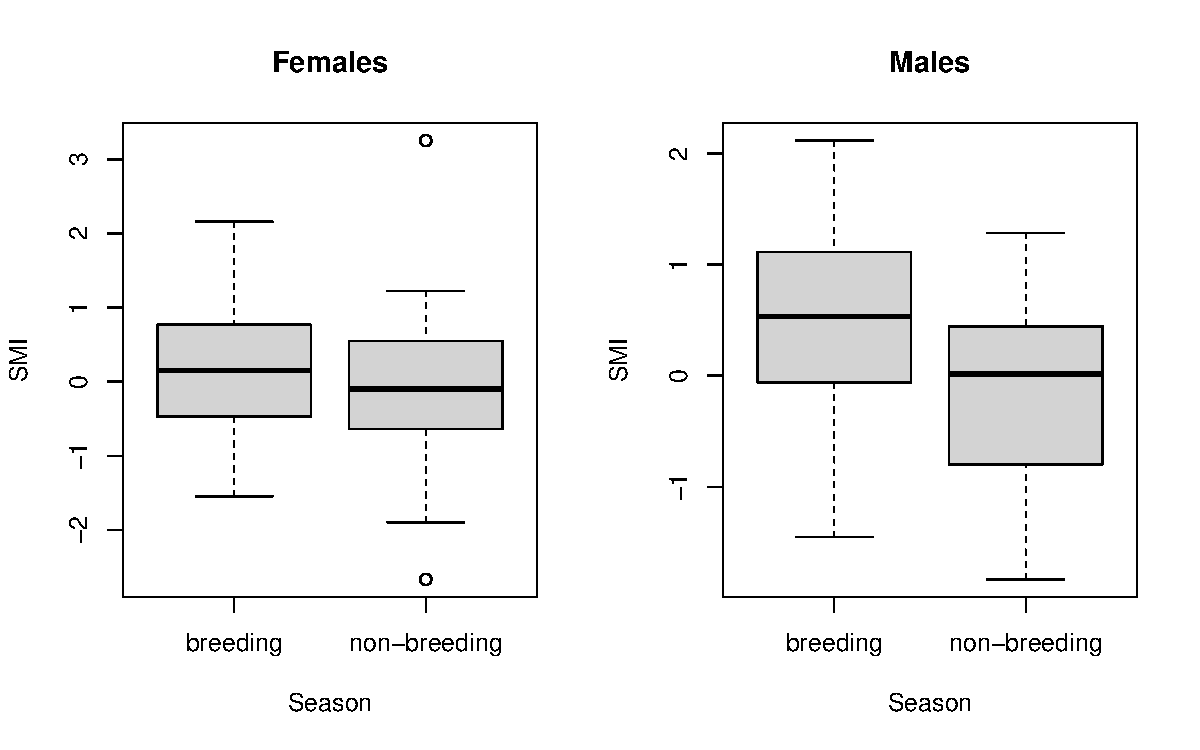
\includegraphics{gcondition_files/figure-latex/p2 condition and season-1.pdf}

Figure 4: Scaled mass index (SMI) was not significantly different
between the breeding and non-breeding seasons for either sex.

Because fat score and SMI did not correlate, we included both as
independent variables in our models testing prediction 2. For both males
and females, we found no statistically significant relationships between
either proxy of energetic condition and reproductive success (Table 3).
Of note, the inconsistent direction of the effects for the parameter
estimates further supports that SMI and fat score do not measure the
same trait.

For females, our SMI parameter estimate of -0.92 (exponentiated to get
the log odds = 0.40) indicates that a one unit increase in SMI
corresponded to a 60\% decrease in the odds a female would fledge an
offspring (\emph{p} = 0.13). Whereas an increase from no visible fat to
showing some fat corresponded to a 16\% increase in the odds a female
would fledge an offspring (log odds = 1.16, \emph{p} = 0.82). There was
also no evidence of a significant relationship between the ability of a
female to produce fledglings and having previously spent time in the
aviaries (log odds = 0.25, \emph{p} = 0.22), where the odds that a
female would fledge an offspring were 75\% lower if females spent time
in the aviaries.

For males, there was also no statistically significant support for a
relationship between whether a male defended a territory and SMI (log
odds = 3.25, \emph{p} = 0.13). Nevertheless, this relationship may be
biologically important because a one unit increase in SMI corresponded
to a more than 300\% increase in the odds a male will hold a territory
containing nests. Fat score was also statistically unrelated to male
reproductive success where an increase from showing no visible fat to
showing some fat corresponded to a 28\% decrease in territory holding
(log odds = 0.72, \emph{p} = 0.76). Lastly, we found that those males
who spent time in the aviaries were statistically less likely (97\%
decrease in the odds) to hold a territory compared with males who were
never in the aviaries (log odds = 0.03, \emph{p} = 0.02). However, we
stress that our sample size was relatively small (20 males), and we did
not have a balanced sample because there were no males that did not
defend a territory and were never in the aviaries. Additionally, only
five males had data from more than one breeding season, which resulted
in our model fit being singular because the random effect for bird ID
accounted for essentially zero variance. However, we kept ID in the
model to account for the repeated samples.

\begin{table}

\caption{\label{tab:p2 main results}Table 3. Results from the logistic regression for 20 females and 20 males to test whether reproductive success relates to condition. Estimates are presented with the standard error in parentheses.}
\centering
\begin{tabular}[t]{lcccc}
\toprule
\multicolumn{1}{c}{ } & \multicolumn{2}{c}{Females} & \multicolumn{2}{c}{Males} \\
\cmidrule(l{3pt}r{3pt}){2-3} \cmidrule(l{3pt}r{3pt}){4-5}
Parameter & Estimate (SE) & p-value & Estimate (SE) & p-value\\
\midrule
Intercept & -0.02 (0.73) & 0.98 & 3.05 (1.40) & 0.03\\
FatScore & 0.15 (1.02) & 0.89 & -0.33 (1.10) & 0.77\\
SMI & -0.92 (0.61) & 0.13 & 1.18 (0.78) & 0.13\\
Aviary & -1.38 (1.14) & 0.23 & -3.62 (1.56) & 0.02*\\
\bottomrule
\end{tabular}
\end{table}

\textbf{Prediction 2: energetic condition and probability of daily nest
survival}

Logistic regression analyses to determine reproductive success from
nests discovered in different stages will be systematically biased
(Shaffer, 2004). Nests discovered at a more progressed stage (i.e.,
nestling stage compared to building stage) are statistically more likely
to succeed and nests with frequent and prolonged adult visits (such as
those that occur when nests survive longer) are more likely to be
discovered. Therefore, nests that fail early are less likely to be
detected (Shaffer, 2004). Consequently, we analyzed female reproductive
success using a logistic exposure model (Bolker, 2014), which uses
survival analysis to determine the factors affecting the probability of
daily nest survival, while accounting for incomplete nest observations.

We found that the probability of daily nest survival was significantly
negatively related to SMI (log odds = 0.50, \emph{p} = 0.03; Table 4),
where, for every unit increase in SMI, the odds of daily nest survival
decreased by half. This indicates that a female with a larger SMI (more
mass for her structural body size) was less likely to have her nest
survive each day (Fig. 5). There was no statistically significant
relationship between the probability of daily nest survival and fat
score (log odds = 2.48, \emph{p} = 0.06), day of the year (log odds =
0.81, \emph{p} = 0.16), or time spent in the aviaries (log odds = 0.63,
\emph{p} = 0.44, Table 4). Although not statistically significant, the
effect size for the relationship between fat score and daily nest
survival is large (Fig. 5) and potentially biologically meaningful. The
odds of a nest surviving on a given day are almost 2.5 times greater
(248\%) for birds with some fat (a score of 1) compared to no fat (a
score of 0).

\begin{table}

\caption{\label{tab:logexp}Table 4. Results of the logistic exposure model showing the relationship between the probability of daily nest survival and scaled mass index (SMI), fat score, the amount of time spent in the aviaries, and the day of the year. Parameter estimates are presented with the standard error in parentheses. Odds ratios (OR) represent the exponentiated estimates, and are presented to increase interpretability with 95 percent confidence intervals in parentheses.}
\centering
\begin{tabular}[t]{lccc}
\toprule
Parameter & Estimate (SE) & OR (CI) & p-value\\
\midrule
Intercept & 1.99 (0.40) & 7.32 (3.3-16.0) & <0.001\\
Fat score & 0.91 (0.49) & 0.50 (0.27-0.92) & 0.06\\
SMI & -0.69 (0.31) & 2.48 (0.95-6.49) & 0.03*\\
Day of year & -0.21 (0.15) & 0.63 (0.19-2.10) & 0.16\\
Aviary & -0.47 (0.61) & 0.81 (0.60-1.10) & 0.44\\
\bottomrule
\end{tabular}
\end{table}

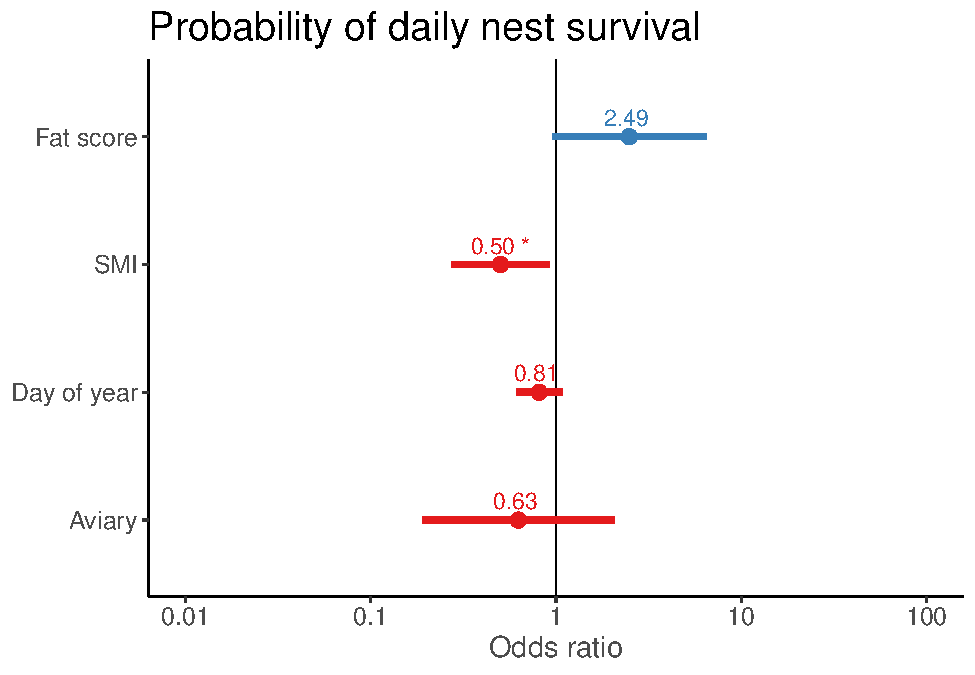
\includegraphics{gcondition_files/figure-latex/logoddfig-1.pdf}

Figure 5: Odds ratios for independent variables affecting the
probability of a nest surviving a given day. The dots and corresponding
values represent the odds ratio values, and lines represent the
confidence intervals around the odds ratio value. The vertical line at x
= 1 delineates the odds ratio value for no relationship between the
estimates and the probability of daily nest survival. The asterisk
indicates an odds ratio value that is statistically significant.

\hypertarget{discussion}{%
\section{DISCUSSION}\label{discussion}}

Energetic condition is not directly observable, but variation can affect
life history characteristics (Barnett et al., 2015; Labocha et al.,
2014). Consequently, a large corpus of research attempts to measure
energetic condition using various proxy measures (Labocha et al., 2014)
and largely assumes that the chosen proxy accurately reflects energetic
condition as a singular trait. Although it is often implicitly assumed
that all proxy measures for energetic condition reflect the same
inherent trait, it is rare for one study to compare multiple proxies.
However, if all proxy measures are affected similarly by a singular
energetic condition phenotype, then multiple proxy measures should
produce correlated results. The aim of the current study was therefore
to test the idea that multiple commonly used morphological proxies
equally measure energetic condition (by correlating with each other),
and that these measures can explain variation in reproductive success.

Here we found that two morphological proxies of energetic condition, fat
score and SMI, did not correlate with each other in the great-tailed
grackle, regardless of whether it was the breeding or non-breeding
season. While both proxies are well supported in previous research as
measures of energetic condition, our results indicate that they may not
be measuring the same trait. This has also been found in studies on bats
(McGuire et al., 2018), which are species that similarly experience
distinct demands on body structure to facilitate flight. There are
several potential reasons why grackle fat score and SMI did not
correlate. First, it is possible that we were unable to accurately
measure the amount of fat the birds actually stored. In addition to
storing fat under their skin, birds may also store fat intraperitoneally
(Musacchia, 1953), which would not have been detected with our fat score
measure. Second, SMI and fat score may measure different components of
energetic condition because variation in mass among grackles could be
attributable to muscle or body water content, whereas fat score only
accounts for subcutaneous fat (Labocha \& Hayes, 2012). Research shows
that stored fat is the primary source of energy in many taxa (Walsberg,
1988), especially in birds (Blem, 1990; Pond, 1981) because the energy
per ounce from fat is much higher than from proteins or carbohydrates
(Gessaman, 1999). However, because desert birds, such as the grackles in
our investigation, have inconsistent access to water sources, variation
in body water content may obscure variation in lipid content. Measuring
muscle content often requires destructive methods {[}i.e.~sacrificing
the birds; Zhang et al. (2015){]} or less objective assessments such as
keel prominence or breast muscle shape (Abolins-Abols \& Ketterson,
2017; A. Gosler, 1991), which was beyond the scope of the current
research program. Third, it is possible that fat score and SMI did not
correlate due to temporal variation at a fine scale that we were unable
to capture. Although we found no evidence that SMI or fat score varied
by season, there is evidence from other studies that avian mass changes
with time of day (Nip et al., 2019) and stage of breeding (Milenkaya et
al., 2013). It was logistically impossible in our project (and in many
avian research programs) to capture birds multiple times within a season
or at several times per day, therefore temporal variation in data
collection could obscure the correlation between these two proxies, if
such a correlation exists. However, the stage of breeding is unlikely to
introduce additional variance to our study because we did not catch any
females that were actively engaged in any stage of the breeding process.
Finally, our sample sizes might have been too small to detect an effect,
but the effect size for the relationship between fat score and SMI was
essentially zero (0.001), therefore it is unlikely that a larger sample
size would find a biologically informative relationship between these
two proxies.

Energetic condition can have a large impact on reproductive success in
birds (Drent \& Daan, 1980; Montreuil-Spencer, 2017) and in flying
mammals (Welbergen, 2011). For example, female chickadees with higher
winter fat scores are more likely to lay eggs earlier in the subsequent
breeding season, as well as go on to feed those offspring more
frequently (Montreuil-Spencer, 2017). Energetic condition is likely a
factor in reproductive success in our system because previous research
in great-tailed grackles found that larger and heavier males were more
likely to hold territories, have more social mates, and sire more
offspring (Johnson et al., 2000). Our study additionally considered
female morphology and reproductive success, subcutaneous fat, and
controlled for the impact of structural body size on mass. However, we
found reproductive success, measured as the ability to produce
fledglings (females) or to hold a territory containing nests (males),
did not significantly correlate with fat score or SMI. Although our
results were not statistically significant, in some cases the parameter
estimates revealed log-odds that may be large enough to be biologically
significant. Notably, a one unit increase in SMI corresponded to a more
than 300\% increase in the odds a male will hold a territory containing
nests, but a 60\% decrease in the odds a female would fledge an
offspring.

We additionally used logistic exposure models to determine whether the
energetic condition of females related to the probability of daily nest
survival. We only included females in this analysis because males were
never observed contributing to nest building, incubation, or feeding
nestlings in our population and so will not have a direct effect on
daily nest survival. We found a negative relationship between female SMI
and the likelihood of daily nest survival. This could be due to larger
females actually carrying proportionally smaller energetic reserves than
their smaller female counterparts (Jacobs et al., 2012), as seen in
red-winged blackbirds (Langston et al., 1990). In some species, females
with smaller body sizes are able to initiate breeding earlier because
they can allocate more resources to reproduction compared to larger
individuals that have higher bodily energy demands and therefore fewer
excess energetic resources (Barbraud et al., 2000; Langston et al.,
1990; Murphy, 1986). This indirectly affects reproductive success
because nesting earlier increases the probability of nesting success and
multiple nesting attempts (Johnson \& Peer, 2001; Perrins, 1970). Yet,
in our study we found no relationship between the probability of daily
nest survival and day of the year, therefore this is unlikely to explain
the negative relationship between SMI and nest survival. Alternatively,
it is possible that larger females are unable to build a more concealed
nest in the most dense vegetation, or that larger females are unable to
build nests in delicate vegetation structure that is more likely to be
inaccessible to predators. Moreover, the parameter estimate for the
relationship between fat score and the daily probability of nest
survival indicates that females with some visible fat are more than
twice as likely to have a nest survive a given day. Because the
direction of this effect is opposite to the relationship between SMI and
nest survival, this is further evidence that these two proxies represent
different traits.

Great-tailed grackles are an interesting system to study energetic
condition and reproductive success because they recently expanded their
range into Arizona, where the climate and habitat are distinct from that
in Central America where the species originally evolved (Wehtje, 2003).
The increase in temperature variation and decrease in available water at
our desert study site are both environmental stressors that have
previously been found to negatively affect energetic condition
(Pendlebury et al., 2004). Although our study spanned only two years,
our data are likely representative of reproductive success in this
environment because the temperatures during our study were in line with
those from the previous three years (National Climatic Data Center,
2020). Reproductive success is vital to species persistence and
abundance in novel environments (Maspons et al., 2019). Therefore, an
understanding of energetic condition and its relationship with
reproductive success in grackles outside of their original range could
broadly inform conservation research in invasive and non-native species.
While reproductive success of certain avian species may be easier to
monitor at a more fine scale (i.e.~cavity nesters), the predominant
measure of reproductive success currently used by avian ecologists is
the ability of adults to fledge offspring (since foundational work by
Mayfield, 1961) because it is financially and logistically accessible to
more researchers. Therefore, we believe our measure of reproductive
success in grackles is informative, and that research that spans taxa
with diverse reproductive strategies is important for understanding
general trends in energetic condition and the appropriate proxies.

The results of this study highlight the need to better understand proxy
measures of energetic condition, not only in grackles, but for birds in
general. Most studies on avian energetic condition only use one proxy
variable, but because energetic condition is difficult to measure
directly, it is important to compare multiple proxy variables to
determine whether the proxy is measuring the intended trait (Block,
1995; Carter et al., 2013). If financially and logistically feasible,
future research could measure total body composition and relative mass
of fat using the relatively new and promising method of quantitative
magnetic resonance (Guglielmo et al., 2011), or researchers could
incorporate additional physiological methods to measure energetic
condition, for example, blood hematocrit levels (Dawson \& Bortolotti,
1997; but see Fair et al., 2007). Additionally, studying traits that
could relate to variation in energy stores, such as dispersal (Ellers et
al., 1998), migratory endurance (Deppe et al., 2015), or survival (Liao
et al., 2011) would allow us to disentangle whether morphological
proxies like fat score and SMI are poor proxy measures for energetic
condition, or whether fat score and SMI do not affect reproductive
success but may be associated with other life history characteristics.
Because SMI can perform poorly in birds with low lipid mass, future
research should also compare several mass by structural body size
equations to determine the most appropriate proxy for a specific study
system (Jacobs et al., 2012). Lastly, future research would benefit from
using logistic exposure models to examine the relationship between
energetic condition and reproductive success because these models
control for the bias that arises when early nest failures are not
detected, which is not possible in logistic regression models, and it is
more sensitive to changes in a bird's nest status (Shaffer, 2004).

\pagebreak

\hypertarget{detailed-hypotheses-and-methods-from-the-preregistration}{%
\section{DETAILED HYPOTHESES AND METHODS FROM THE
PREREGISTRATION}\label{detailed-hypotheses-and-methods-from-the-preregistration}}

\hypertarget{hypotheses-1}{%
\subsubsection{HYPOTHESES}\label{hypotheses-1}}

We measured two morphological proxy variables of energetic condition and
observed reproductive success in grackles to test two hypotheses:

\textbf{H1 - There is a relationship between two different morphological
indices of energetic condition: fat score and the scaled mass index.}

\textbf{Prediction 1:} Fat score and the scaled mass index will be
positively correlated. This would indicate that these two indices
measure the same trait, and it is likely they both are proxies for fat
content.

\textbf{Prediction 1 alternative 1:} There is a negative correlation
between fat score and the scaled mass index. This would indicate that
there may be a tradeoff between the two indices where a larger value of
the scaled mass index may measure muscle content rather than fat, and
individuals with more muscle have less visible fat.

\textbf{Prediction 1 alternative 2:} There is no correlation between fat
score and the scaled mass index. This indicates that these two variables
do not measure the same trait. Fat score may not adequately capture a
bird's energetic condition because birds may be selected to only store
the minimal fat necessary to prevent starvation, while also minimizing
the weight gain that would make them easier targets for predators
(Barnett et al., 2015). Similarly, the scaled mass index could be
heavily influenced by body size, therefore reflecting structural size
rather than fat storage (Labocha \& Hayes, 2012).

\textbf{H2 - Energetic condition (as measured by fat score and the
scaled mass index) relates to reproductive success (measured as a binary
variable of whether a female had one or more fledglings (1) or not (0),
and whether a male defended a territory containing nests (1) or not
(0)).}

\textbf{Prediction 2:} Morphological indices of energetic condition (fat
score and the scaled mass index) will correlate positively with
reproductive success. This would indicate that individuals with more
fat, and therefore higher energy reserves, are better able to acquire
the resources necessary for reproduction.

\textbf{Prediction 2 alternative 1:} Morphological indices of energetic
condition (fat score and the scaled mass index) will correlate
negatively with reproductive success. This indicates that individuals
may make trade offs, with some acquiring more food and increasing their
energy reserves, and others prioritizing reproductive activities over
increasing energy reserves.

\textbf{Prediction 2 alternative 2:} Morphological indices of energetic
condition (fat score and the scaled mass index) do not correlate with
reproductive success. This indicates that other, potentially
non-morphological, individual characteristics relate to reproductive
success (i.e., cognition, nest site selection, breeding experience,
predator vigilance, etc.).

\hypertarget{methods-1}{%
\subsubsection{METHODS}\label{methods-1}}

The methods below are based on the preregistration, with small changes
as described in the
\protect\hyperlink{associated-preregistration}{Deviations from the
planned methods} section above.

\hypertarget{planned-sample}{%
\paragraph{\texorpdfstring{\textbf{Planned
Sample}}{Planned Sample}}\label{planned-sample}}

Great-tailed grackles are caught in the wild in Tempe, Arizona using a
variety of methods (e.g., walk-in trap, bownet, mist net). After capture
we immediately process birds by attaching colored leg bands in unique
combinations for individual identification, conducting morphological
measurements of weight, tarsus length, flattened wing length, tail
length, skull length, bill length and fat score (the amount of visible
fat under the skin in the clavicle and abdomen as in Kaiser, 1993). Most
grackles are released after completion of color band marking,
measurements, and acquiring a blood sample. A subset of grackles are
held in aviaries for up to 6 months for behavioral testing, and then
released back to the wild at their location of capture.

From March - August, we monitor the behavior of all color-marked
grackles to determine their nesting status. We follow females carrying
nesting materials to find their nest. We determine whether the male
territory owner is color-marked as well. Then we check each nest
approximately every day to determine the status based on the female's
behavior (building, incubation, feeding nestlings, feeding fledglings,
failed).

Individuals included in this sample will be those for which we have
measures of energetic condition when they were adults. We will not
include individuals whose data were collected as juveniles. As of 30
July 2019, we have fledgling data for 14 females that exhibited breeding
behavior (5 had 1+ fledgling, 9 had no fledglings) and breeding
territory status for 10 males (7 territory holders, 3 non-territory
holders, 2 not observed so not part of this sample). Therefore, the
minimum sample size for H2 will be 24. The minimum sample size for H1
will be 72, because that is how many marked individuals we have
biometric data for so far. However, we expect to be able to add to the
sample size for both H1 and H2 before the end of this investigation in
Tempe, Arizona. \emph{UPDATE Oct 2020: In the second breeding season we
had 20 females and 20 males with reproductive success and energetic
condition data.}

\hypertarget{sample-size-rationale}{%
\paragraph{\texorpdfstring{\textbf{Sample size
rationale}}{Sample size rationale}}\label{sample-size-rationale}}

We will continue to color mark as many grackles as possible, and collect
biometric data and fat scores. Our current sample of reproductive
success is small because the grackles in Tempe nest in very tall palms,
making it difficult to determine nest status. However, we plan to
collect additional reproductive success data during the breeding season
in summer 2020. \emph{UPDATE Oct 2020: In the second breeding season we
had 20 females and 20 males with reproductive success and energetic
condition data.}

\hypertarget{data-collection-stopping-rule}{%
\paragraph{\texorpdfstring{\textbf{Data collection stopping
rule}}{Data collection stopping rule}}\label{data-collection-stopping-rule}}

We will stop collecting data for this project in early August 2020 when
research at the Tempe, Arizona field site will be finished.

\hypertarget{open-materials}{%
\paragraph{\texorpdfstring{\textbf{Open
materials}}{Open materials}}\label{open-materials}}

Biometric measurement protocol:
\url{https://gitlab.com/corinalogan/the-grackle-project/blob/master/protocolBiometrics.pdf}

Nest check protocol:
\url{https://gitlab.com/corinalogan/the-grackle-project/blob/master/protocolNestCheck.pdf}

\hypertarget{open-data}{%
\paragraph{\texorpdfstring{\textbf{Open
data}}{Open data}}\label{open-data}}

All data (Berens et al., 2020) are available at
\url{https://knb.ecoinformatics.org/view/doi:10.5063/F1NZ862D} and at
github (the provided code will load these files directly from github).

\hypertarget{randomization-and-counterbalancing}{%
\paragraph{\texorpdfstring{\textbf{Randomization and
counterbalancing}}{Randomization and counterbalancing}}\label{randomization-and-counterbalancing}}

There is no randomization or counterbalancing in this investigation.

\hypertarget{blinding-of-conditions-during-analysis}{%
\paragraph{\texorpdfstring{\textbf{Blinding of conditions during
analysis}}{Blinding of conditions during analysis}}\label{blinding-of-conditions-during-analysis}}

No blinding is involved in this investigation.

\textbf{Dependent Variables}

\textbf{P1: correlation between fat and the scaled mass index}

\begin{enumerate}
\def\labelenumi{\arabic{enumi})}
\tightlist
\item
  Fat score {[}the amount of visible fat under the skin in the clavicle
  and abdomen reported as a score from 0 (no fat) to 8 (fat completely
  covers muscles and underside of the bird); Kaiser (1993){]}
  \emph{UPDATE Oct 2020: Fat score was heavily 0 skewed with few scores
  greater than one. To increase model fit we used a binomial response
  variable instead, where 0 is no fat and 1 is some fat observed undert
  the skin.}
\end{enumerate}

\textbf{P2: energetic condition and reproductive success}

\begin{enumerate}
\def\labelenumi{\arabic{enumi})}
\item
  Female had one or more fledglings (yes, no)
\item
  Male held a territory consisting of 1 to 3 clumped palms containing
  nests (yes, no)
\end{enumerate}

\textbf{Independent Variables}

\textbf{P1: correlation between fat and the scaled mass index}

\begin{enumerate}
\def\labelenumi{\arabic{enumi})}
\item
  Scaled mass index using measures of body weight and tarsus length or
  flattened wing length (average of left and right as in Bleeker et al.,
  2005). We will choose the measure that is most correlated with body
  weight (Peig \& Green, 2009).
\item
  Season (non-breeding {[}Sep-Feb{]}, breeding {[}Mar-Aug{]}).
  \emph{UPDATE Oct 2020: The Season variable only includes 2 males in
  the breeding season category, thus we do not have a large enough
  sample to produce reliable estimates. We removed the Season variable
  from the model for males.}
\item
  Random effect: Experimenter (because several different experimenters
  measure dependent variables on multiple different birds)
\end{enumerate}

\textbf{P2: energetic condition and reproductive success}

\begin{enumerate}
\def\labelenumi{\arabic{enumi})}
\item
  Fat score

  \begin{itemize}
  \tightlist
  \item
    Note 1: if the fat score and the scaled mass index are positively
    correlated, then we will use only fat score in the model for P2. If
    they are not positively correlated, then we will add the scaled mass
    index as an independent variable in the P2 analysis
  \item
    Note 2: if fat score and/or the scaled mass index vary by season
    (breeding or non-breeding), then we will only use the data from the
    breeding season to ensure that less time has elapsed between the
    collection of energetic condition and reproductive success variables
  \end{itemize}
\item
  Temporarily held in aviaries for behavioral testing at any point
  during this study, because this may affect breeding behaviors (yes,
  no)
\item
  Random effect: Year (to determine whether conditions in a given
  breeding season similarly affected all grackle behavior and nest
  success)
\item
  Random effect: Bird ID (because there may be multiple measures of
  reproductive success for each bird)
\end{enumerate}

\hypertarget{analysis-plan}{%
\subsubsection{ANALYSIS PLAN}\label{analysis-plan}}

\emph{UPDATE Oct 2020:}

\emph{1) We realized that the sexual dimorphism of male and female body
sizes necessitates separate analyses. Therefore, we calculated SMI for
males and females separately, ran separate models for each sex for the
repeatibility analysis, P1 and P2.}

\emph{2) Fat score data were distributed such that the majority of
scores were 0, with some 1's and very few higher numbers. This made it
difficult to fit models using an ordinal regression. The function
simulateResiduals, which we used to check our data, does not work with
data in the ordinal family. Consequently, we used logistic regression
where the dependent variable FatScore represents no fat (score = 0), or
some fat (score = 1)}

\emph{3) Despite the data checking which indicated our model was not
overdispersed or zero inflated, we could not get the fixed effects or
random effect to converge using the Bayesian MCMCglmm. We found no
improvement in model fit by tweaking the priors or
iterations/burnin/thin options. Therefore, we fit these models using the
function glmer, a frequentist framework.}

\emph{4) The Season variable only includes 2 males in the breeding
season category, thus we do not have a large enough sample to produce
reliable estimates. We removed the Season variable from the model for
males.}

We will \textbf{exclude} data that was collected from the grackles when
they were released from the aviaries to avoid any confounds due to their
time in the aviary (e.g., perhaps unlimited nutritious food in the
aviaries affected their fat score). However, to validate that our
measures of structural body size (tarsus length or wing length) are
precise and accurate, we will measure twice a subset of grackles brought
into aviaries - once when they are initially caught, and again up to 6
months later when we release them. We will then calculate the
repeatability of these multiple measures. All other data included in
this study will come only from wild-caught grackles (including the birds
that were brought into the aviaries on their first capture). When
\textbf{missing data} occur, the existing data for that individual will
be included in the analyses for which their data exist. Analyses will be
conducted in R {[}current version 4.0.5; R Core Team (2017){]}.

\hypertarget{ability-to-detect-actual-effects}{%
\paragraph{\texorpdfstring{\emph{Ability to detect actual
effects}}{Ability to detect actual effects}}\label{ability-to-detect-actual-effects}}

To begin to understand what kinds of effect sizes we will be able to
detect given our sample size limitations, we used G*Power Faul et al.
(2009) to conduct power analyses based on confidence intervals. G*Power
uses pre-set drop down menus and we chose the options that were as close
to our analysis methods as possible (listed in each analysis below).
Note that there were no explicit options for GLMMs, thus the power
analyses are only an approximation of the kinds of effect sizes we can
detect. We realize that these power analyses are not fully aligned with
our study design and that these kinds of analyses are not appropriate
for Bayesian statistics (e.g., our MCMCglmm below), however we are
unaware of better options at this time. Additionally, it is difficult to
run power analyses because it is unclear what kinds of effect sizes we
should expect due to the lack of data on this species for these
particular research questions.

\hypertarget{data-checking}{%
\paragraph{\texorpdfstring{\emph{Data
checking}}{Data checking}}\label{data-checking}}

The data will be checked for overdispersion, underdispersion,
zero-inflation, and heteroscedasticity with the DHARMa R package
(Hartig, 2019) following methods by
\href{https://cran.r-project.org/web/packages/DHARMa/vignettes/DHARMa.html}{Hartig}.

\emph{P1 analysis: correlation between fat and the scaled mass index}

We will calculate the scaled mass index as described by Peig \& Green
(2009) using either tarsus or flattened wing length - whichever measure
is most correlated with body weight (Peig \& Green, 2009).

We use a Generalized Linear Mixed Model (GLMM; MCMCglmm function,
MCMCglmm package; (Hadfield 2010)) with an ordinal distribution (for
categorical variables in MCMCglmm) and probit link using 130,000
iterations with a thinning interval of 10, a burnin of 30,000, and
minimal priors (V=1, nu=0) (Hadfield, 2014). We will ensure the GLMM
shows acceptable convergence {[}lag time autocorrelation values
\textless0.01; Hadfield (2010){]}, and adjust parameters if necessary to
meet this criterion. We will determine whether an independent variable
had an effect or not using the Estimate in the full model.

Where we have multiple measures of tarsus or flattened wing length, we
will check that our measurements are repeatable using the rptR package
(Stoffel et al., 2017).

To roughly estimate our ability to detect actual effects (because these
power analyses are designed for frequentist statistics, not Bayesian
statistics), we ran a power analysis in G*Power with the following
settings: test family=F tests, statistical test=linear multiple
regression: Fixed model (R\^{}2 deviation from zero), type of power
analysis=a priori, alpha error probability=0.05. We changed the power
and the effect size until we reached an output that we project our
sample size will be (n=90). The number of predictor variables was
restricted to only the fixed effects because this test was not designed
for mixed models. The protocol of the power analysis is here:

\emph{Input:}

Effect size f² = 0.15

α err prob = 0.05

Power (1-β err prob) = 0.86

Number of predictors = 3

\emph{Output:}

Noncentrality parameter λ = 13.3500000

Critical F = 2.7119214

Numerator df = 3

Denominator df = 85

Total sample size = 89

Actual power = 0.8635760

This means that, with a sample size of 89, we would have an 86\% chance
of detecting a medium effect (approximated at f\textsuperscript{2}=0.15
by Cohen, 1988).

\emph{code shown in .rmd}

\emph{P2 analysis: energetic condition and reproductive success}

To model the effect of energetic condition on reproductive success, we
will use two types of logistic mixed-effect models. Both types are
supported in the literature, but are slightly different in the way in
which the link function is specified. First, we will model reproductive
success using a generalized linear mixed model framework with a logit
link function (i.e. Milenkaya et al., 2015). We will also use a logistic
exposure model that has a link function which accounts for the time
interval between nest checks when estimating the probability of daily
nest survival (Bolker, 2014; Shaffer, 2004). If fat score and the scaled
mass index are positively correlated in P1, then we will use only fat
score as the independent variable in this GLMM. If they are not
positively correlated, we will include both as independent variables.

Previous research found a non-linear relationship between reproductive
success and energetic condition variables (Milenkaya et al., 2015). To
check whether this is occurring in our data, we will first plot our raw
data to determine if we need to include a non-linear energetic condition
independent variable into our model (i.e.~FatScore\textsuperscript{2}).
Our dependent variable is binary, so to more clearly see the trends in
the data, on the x-axis we will bin our energetic condition scores into
5 categories based on standard deviations (sd) around the mean (low =
\textless{} 2 sd, moderately low = -2 sd to -1 sd, moderate = -1 sd to
+1 sd, moderately high = +1 sd to +2 sd, high = \textgreater{} 2 sd).
Then on the y-axis we will use the proportion of individuals in each
category that had successful nests. \emph{UPDATE Oct 2020: Because most
individuals fell within the medium category when we grouped data using 1
standard deviation around the mean, we switched to using half standard
deviation increments around the mean.}

A power analysis was conducted as above for P1 and the protocol reported
here:

\emph{Input:}

Effect size f² = 0.15

α err prob = 0.05

Power (1-β err prob) = 0.90

Number of predictors = 2

\emph{Output:}

Noncentrality parameter λ = 13.2000000

Critical F = 3.1038387

Numerator df = 2

Denominator df = 85

Total sample size = 88

Actual power = 0.9020264

This means that, with a sample size of 88, we would have a 90\% chance
of detecting a medium effect (approximated at f\textsuperscript{2}=0.15
by Cohen, 1988).

\emph{code shown in .rmd}

\hypertarget{do-energetic-condition-variables-vary-by-season}{%
\paragraph{Do energetic condition variables vary by
season?}\label{do-energetic-condition-variables-vary-by-season}}

\emph{code shown in .rmd}

\hypertarget{does-energetic-condition-relate-to-reproductive-success}{%
\paragraph{Does energetic condition relate to reproductive
success?}\label{does-energetic-condition-relate-to-reproductive-success}}

\emph{code shown in .rmd}

\hypertarget{does-female-energetic-condition-relate-to-the-probability-of-daily-nest-survival}{%
\paragraph{Does female energetic condition relate to the probability of
daily nest
survival?}\label{does-female-energetic-condition-relate-to-the-probability-of-daily-nest-survival}}

Our measure of female nest success could be systematically biased
against nests that failed early (Shaffer, 2004). Consequently, we also
analyzed female reproductive success using a logistic exposure model.
This type of model determines the factors affecting daily nest survival
probability.

\emph{code shown in .rmd}

\hypertarget{ethics}{%
\section{ETHICS}\label{ethics}}

This research is carried out in accordance with permits from the:

\begin{enumerate}
\def\labelenumi{\arabic{enumi})}
\tightlist
\item
  US Fish and Wildlife Service (scientific collecting permit number
  MB76700A-0,1,2)
\item
  US Geological Survey Bird Banding Laboratory (federal bird banding
  permit number 23872)
\item
  Arizona Game and Fish Department (scientific collecting license number
  SP594338 {[}2017{]}, SP606267 {[}2018{]}, and SP639866 {[}2019{]})
\item
  Institutional Animal Care and Use Committee at Arizona State
  University (protocol number 17-1594R)
\end{enumerate}

\hypertarget{author-contributions}{%
\section{AUTHOR CONTRIBUTIONS}\label{author-contributions}}

\textbf{Berens:} Hypothesis development, data collection,
revising/editing.

\textbf{Logan:} Study design, write up, revising/editing,
materials/funding.

\textbf{Folsom:} Data collection, revising/editing.

\textbf{Sevchik} Data collection, revising/editing.

\textbf{Bergeron:} Data collection, revising/editing.

\textbf{McCune:} Hypothesis development, data collection, data analysis,
write up, revising/editing.

\hypertarget{funding}{%
\section{FUNDING}\label{funding}}

This research is funded by the Department of Human Behavior, Ecology and
Culture at the Max Planck Institute for Evolutionary Anthropology.

\hypertarget{acknowledgements}{%
\section{ACKNOWLEDGEMENTS}\label{acknowledgements}}

We thank Aaron Blackwell and Ken Kosik for being the UCSB sponsors of
the Cooperation Agreement with the Max Planck Institute for Evolutionary
Anthropology; and our research assistants for help with trapping the
grackles and collecting the biometric and nest/territory data: Aelin
Mayer, Nancy Rodriguez, Brianna Thomas, Aldora Messinger, Elysia Mamola,
Michael Guillen, Rita Barakat, Adriana Boderash, Olateju Ojekunle,
August Sevchik, Justin Huynh, Amanda Overholt, and Michael Pickett.

\hypertarget{references}{%
\section*{REFERENCES}\label{references}}
\addcontentsline{toc}{section}{REFERENCES}

\hypertarget{refs}{}
\begin{CSLReferences}{1}{0}
\leavevmode\hypertarget{ref-abolins2017condition}{}%
Abolins-Abols, M., \& Ketterson, E. D. (2017). Condition explains
individual variation in mobbing behavior. \emph{Ethology},
\emph{123}(8), 495--502.

\leavevmode\hypertarget{ref-aubret2002fat}{}%
Aubret, F., Bonnet, X., Shine, R., \& Lourdais, O. (2002). Fat is sexy
for females but not males: The influence of body reserves on
reproduction in snakes (vipera aspis). \emph{Hormones and Behavior},
\emph{42}(2), 135--147.

\leavevmode\hypertarget{ref-barbraud2000body}{}%
Barbraud, C., Lormée, H., \& LeNevé, A. (2000). Body size and
determinants of laying date variation in the snow petrel pagodroma
nivea. \emph{Journal of Avian Biology}, \emph{31}(3), 295--302.

\leavevmode\hypertarget{ref-barnett2015mass}{}%
Barnett, C. A., Suzuki, T. N., Sakaluk, S. K., \& Thompson, C. F.
(2015). Mass-based condition measures and their relationship with
fitness: In what condition is condition? \emph{Journal of Zoology},
\emph{296}(1), 1--5.

\leavevmode\hypertarget{ref-barry2013macronutrient}{}%
Barry, K. L., \& Wilder, S. M. (2013). Macronutrient intake affects
reproduction of a predatory insect. \emph{Oikos}, \emph{122}(7),
1058--1064.

\leavevmode\hypertarget{ref-berens2020conditiondata}{}%
Berens, J., Logan, C., Folsom, M., Sevchik, A., Bergeron, L., \& McCune,
K. (2020). Validating morphological condition indices and their
relationship with reproductive success in great-tailed grackles.
\emph{Knowledge Network for Biocomplexity}, \emph{Data package}.
\url{https://doi.org/10.5063/7P8WSM}

\leavevmode\hypertarget{ref-bleeker2005body}{}%
Bleeker, M., Kingma, S. A., Szentirmai, I., Székely, T., \& Komdeur, J.
(2005). Body condition and clutch desertion in penduline tit remiz
pendulinus. \emph{Behaviour}, \emph{142}, 1465--1478.

\leavevmode\hypertarget{ref-blem1990avian}{}%
Blem, C. (1990). Avian energy storage. \emph{Curr Ornithol}, \emph{7},
59--113.

\leavevmode\hypertarget{ref-block1995contrarian}{}%
Block, J. (1995). A contrarian view of the five-factor approach to
personality description. \emph{Psychological Bulletin}, \emph{117}(2),
187.

\leavevmode\hypertarget{ref-bolker2014logistic}{}%
Bolker, B. (2014). Logistic regression, accounting for differences in
exposure. \emph{Version 09.30. 2014. RPubs}.

\leavevmode\hypertarget{ref-carter2013animal}{}%
Carter, A. J., Feeney, W. E., Marshall, H. H., Cowlishaw, G., \&
Heinsohn, R. (2013). Animal personality: What are behavioural ecologists
measuring? \emph{Biological Reviews}, \emph{88}(2), 465--475.

\leavevmode\hypertarget{ref-champagnon2012low}{}%
Champagnon, J., Guillemain, M., Elmberg, J., Massez, G., Cavallo, F., \&
Gauthier-Clerc, M. (2012). Low survival after release into the wild:
Assessing {``the burden of captivity''} on mallard physiology and
behaviour. \emph{European Journal of Wildlife Research}, \emph{58}(1),
255--267.

\leavevmode\hypertarget{ref-cohen1988statistical}{}%
Cohen, J. (1988). \emph{Statistical power analysis for the behavioral
sciences 2nd edn}. Erlbaum Associates, Hillsdale.

\leavevmode\hypertarget{ref-cornelius2019physiological}{}%
Cornelius Ruhs, E., Vézina, F., \& Karasov, W. H. (2019). Physiological
and immune responses of free-living temperate birds provided a gradient
of food supplementation. \emph{Physiological and Biochemical Zoology},
\emph{92}(1), 106--114.

\leavevmode\hypertarget{ref-costa2012behavioural}{}%
Costa, G. (2012). \emph{Behavioural adaptations of desert animals}.
Springer Science \& Business Media.

\leavevmode\hypertarget{ref-dawson1997avian}{}%
Dawson, R. D., \& Bortolotti, G. R. (1997). Are avian hematocrits
indicative of condition? American kestrels as a model. \emph{The Journal
of Wildlife Management}, 1297--1306.

\leavevmode\hypertarget{ref-delciellos2018habitat}{}%
Delciellos, A. C., Barros, C. dos S. de, Prevedello, J. A., Ferreira, M.
S., Cerqueira, R., \& Vieira, M. V. (2018). Habitat fragmentation
affects individual condition: Evidence from small mammals of the
brazilian atlantic forest. \emph{Journal of Mammalogy}, \emph{99}(4),
936--945.

\leavevmode\hypertarget{ref-deppe2015fat}{}%
Deppe, J. L., Ward, M. P., Bolus, R. T., Diehl, R. H., Celis-Murillo,
A., Zenzal, T. J., Moore, F. R., Benson, T. J., Smolinsky, J. A.,
Schofield, L. N., \& others. (2015). Fat, weather, and date affect
migratory songbirds' departure decisions, routes, and time it takes to
cross the gulf of mexico. \emph{Proceedings of the National Academy of
Sciences}, \emph{112}(46), E6331--E6338.

\leavevmode\hypertarget{ref-drent1980prudent}{}%
Drent, R., \& Daan, S. (1980). The prudent parent: Energetic adjustments
in avian breeding 1. \emph{Ardea}, \emph{55}(1--2), 225--252.

\leavevmode\hypertarget{ref-ellers1998field}{}%
Ellers, J., Van Alphen, J. J., \& Sevenster, J. G. (1998). A field study
of size--fitness relationships in the parasitoid asobara tabida.
\emph{Journal of Animal Ecology}, \emph{67}(2), 318--324.

\leavevmode\hypertarget{ref-english2018body}{}%
English, M. D., Robertson, G. J., Peck, L. E., Pirie-Hay, D., Roul, S.,
\& Mallory, M. L. (2018). Body condition of american black ducks (anas
rubripes) wintering in atlantic canada using carcass composition and a
scaled mass index. \emph{Canadian Journal of Zoology}, \emph{96}(10),
1137--1144.

\leavevmode\hypertarget{ref-erciyas2010body}{}%
Erciyas, K., Gürsoy, A., Özsemir, A., \& Barış, Y. (2010). Body mass and
fat score changes in recaptured birds during the autumn migration at the
cernek ringing station in turkey. \emph{The Ring}, \emph{32}(1-2),
3--15.

\leavevmode\hypertarget{ref-fair2007sources}{}%
Fair, J., Whitaker, S., \& Pearson, B. (2007). Sources of variation in
haematocrit in birds. \emph{Ibis}, \emph{149}(3), 535--552.

\leavevmode\hypertarget{ref-faul2009statistical}{}%
Faul, F., Erdfelder, E., Buchner, A., \& Lang, A.-G. (2009). Statistical
power analyses using g* power 3.1: Tests for correlation and regression
analyses. \emph{Behavior Research Methods}, \emph{41}(4), 1149--1160.

\leavevmode\hypertarget{ref-faul2007g}{}%
Faul, F., Erdfelder, E., Lang, A.-G., \& Buchner, A. (2007). G* power 3:
A flexible statistical power analysis program for the social,
behavioral, and biomedical sciences. \emph{Behavior Research Methods},
\emph{39}(2), 175--191.

\leavevmode\hypertarget{ref-gessaman1999evaluation}{}%
Gessaman, J. (1999). Evaluation of some nonlethal methods of estimating
avian body fat and lean mass. \emph{Proceedings of the 22nd
International Ornithological Congress. University of Natal Press,
Durban}, 2--16.

\leavevmode\hypertarget{ref-gill1995ornithology}{}%
Gill, F. (1995). \emph{Ornithology}. Freeman; Company.

\leavevmode\hypertarget{ref-gosler1991use}{}%
Gosler, A. (1991). On the use of greater covert moult and pectoral
muscle as measures of condition in passerines with data for the great
tit parus major. \emph{Bird Study}, \emph{38}(1), 1--9.

\leavevmode\hypertarget{ref-gosler1995predation}{}%
Gosler, A. G., Greenwood, J. J., \& Perrins, C. (1995). Predation risk
and the cost of being fat. \emph{Nature}, \emph{377}(6550), 621--623.

\leavevmode\hypertarget{ref-guglielmo2011simple}{}%
Guglielmo, C. G., McGuire, L. P., Gerson, A. R., \& Seewagen, C. L.
(2011). Simple, rapid, and non-invasive measurement of fat, lean, and
total water masses of live birds using quantitative magnetic resonance.
\emph{Journal of Ornithology}, \emph{152}(1), 75.

\leavevmode\hypertarget{ref-haas1998effects}{}%
Haas, C. A. (1998). Effects of prior nesting success on site fidelity
and breeding dispersal: An experimental approach. \emph{The Auk},
\emph{115}(4), 929--936.

\leavevmode\hypertarget{ref-hadfield2010mcmc}{}%
Hadfield, J. (2010). MCMC methods for multi-response generalized linear
mixed models: The MCMCglmm r package. \emph{Journal of Statistical
Software}, \emph{33}(2), 1--22.

\leavevmode\hypertarget{ref-hadfield2014coursenotes}{}%
Hadfield, J. (2014). \emph{MCMCglmm course notes}.
\url{http://cran.r-project.org/web/packages/MCMCglmm/vignettes/CourseNotes.pdf}

\leavevmode\hypertarget{ref-Hartig2019dharma}{}%
Hartig, F. (2019). \emph{DHARMa: Residual diagnostics for hierarchical
(multi-level / mixed) regression models}.
\url{http://florianhartig.github.io/DHARMa/}

\leavevmode\hypertarget{ref-heidinger2010patch}{}%
Heidinger, I. M. M., Hein, S., \& Bonte, D. (2010). Patch connectivity
and sand dynamics affect dispersal-related morphology of the blue-winged
grasshopper oedipoda caerulescens in coastal grey dunes. \emph{Insect
Conservation and Diversity}, \emph{3}(3), 205--212.

\leavevmode\hypertarget{ref-henderson2017glucocorticoids}{}%
Henderson, L., Evans, N., Heidinger, B., Herborn, K., \& Arnold, K.
(2017). Do glucocorticoids predict fitness? Linking environmental
conditions, corticosterone and reproductive success in the blue tit,
cyanistes caeruleus. \emph{Royal Society Open Science}, \emph{4}(10),
170875.

\leavevmode\hypertarget{ref-huxley1932problems}{}%
Huxley, J. (1932). \emph{Problems of relative growth}. Dover
Publications.

\leavevmode\hypertarget{ref-jacobs2012determining}{}%
Jacobs, S. R., Elliott, K., Guigueno, M. F., Gaston, A. J., Redman, P.,
Speakman, J. R., \& Weber, J.-M. (2012). Determining seabird body
condition using nonlethal measures. \emph{Physiological and Biochemical
Zoology}, \emph{85}(1), 85--95.

\leavevmode\hypertarget{ref-johnson2000male}{}%
Johnson, K., DuVal, E., Kielt, M., \& Hughes, C. (2000). Male mating
strategies and the mating system of great-tailed grackles.
\emph{Behavioral Ecology}, \emph{11}(2), 132--141.

\leavevmode\hypertarget{ref-johnson2001great}{}%
Johnson, K., \& Peer, B. D. (2001). \emph{Great-tailed grackle:
Quiscalus mexicanus}. Birds of North America, Incorporated.

\leavevmode\hypertarget{ref-kaiser1993new}{}%
Kaiser, A. (1993). A new multi-category classification of subcutaneous
fat deposits of songbirds (una nueva clasificaci{ó}n, con
multi-categor{ı́}as, para los dep{ó}sitos de grasa en aves canoras).
\emph{Journal of Field Ornithology}, 246--255.

\leavevmode\hypertarget{ref-kelly2014evaluating}{}%
Kelly, C. D., Tawes, B. R., \& Worthington, A. M. (2014). Evaluating
indices of body condition in two cricket species. \emph{Ecology and
Evolution}, \emph{4}(23), 4476--4487.

\leavevmode\hypertarget{ref-labocha2012morphometric}{}%
Labocha, M. K., \& Hayes, J. P. (2012). Morphometric indices of body
condition in birds: A review. \emph{Journal of Ornithology},
\emph{153}(1), 1--22.

\leavevmode\hypertarget{ref-labocha2014body}{}%
Labocha, M. K., Schutz, H., \& Hayes, J. P. (2014). Which body condition
index is best? \emph{Oikos}, \emph{123}(1), 111--119.

\leavevmode\hypertarget{ref-langston1990evolution}{}%
Langston, N. E., Freeman, S., Rohwer, S., \& Gori, D. (1990). The
evolution of female body size in red-winged blackbirds: The effects of
timing of breeding, social competition, and reproductive energetics.
\emph{Evolution}, \emph{44}(7), 1764--1779.

\leavevmode\hypertarget{ref-liao2011fat}{}%
Liao, C.-Y., Rikke, B. A., Johnson, T. E., Gelfond, J. A., Diaz, V., \&
Nelson, J. F. (2011). Fat maintenance is a predictor of the murine
lifespan response to dietary restriction. \emph{Aging Cell},
\emph{10}(4), 629--639.

\leavevmode\hypertarget{ref-maceda2014scaled}{}%
Maceda-Veiga, A., Green, A. J., \& De Sostoa, A. (2014). Scaled
body-mass index shows how habitat quality influences the condition of
four fish taxa in north-eastern spain and provides a novel indicator of
ecosystem health. \emph{Freshwater Biology}, \emph{59}(6), 1145--1160.

\leavevmode\hypertarget{ref-maspons2019behaviour}{}%
Maspons, J., Molowny-Horas, R., \& Sol, D. (2019). Behaviour, life
history and persistence in novel environments. \emph{Philosophical
Transactions of the Royal Society B}, \emph{374}(1781), 20180056.

\leavevmode\hypertarget{ref-mayfield1961nesting}{}%
Mayfield, H. (1961). Nesting success calculated from exposure. \emph{The
Wilson Bulletin}, 255--261.

\leavevmode\hypertarget{ref-mcguire2018common}{}%
McGuire, L. P., Kelly, L. A., Baloun, D. E., Boyle, W. A., Cheng, T. L.,
Clerc, J., Fuller, N. W., Gerson, A. R., Jonasson, K. A., Rogers, E. J.,
\& others. (2018). Common condition indices are no more effective than
body mass for estimating fat stores in insectivorous bats. \emph{Journal
of Mammalogy}, \emph{99}(5), 1065--1071.

\leavevmode\hypertarget{ref-mcnamara2005theoretical}{}%
McNamara, J. M., Barta, Z., Houston, A. I., \& Race, P. (2005). A
theoretical investigation of the effect of predators on foraging
behaviour and energy reserves. \emph{Proceedings of the Royal Society B:
Biological Sciences}, \emph{272}(1566), 929--934.

\leavevmode\hypertarget{ref-merila1997fat}{}%
Merilä, J., \& Svensson, E. (1997). Are fat reserves in migratory birds
affected by condition in early life? \emph{Journal of Avian Biology},
279--286.

\leavevmode\hypertarget{ref-milenkaya2015body}{}%
Milenkaya, O., Catlin, D. H., Legge, S., \& Walters, J. R. (2015). Body
condition indices predict reproductive success but not survival in a
sedentary, tropical bird. \emph{PLoS One}, \emph{10}(8), e0136582.

\leavevmode\hypertarget{ref-milenkaya2013variation}{}%
Milenkaya, O., Weinstein, N., Legge, S., \& Walters, J. R. (2013).
Variation in body condition indices of crimson finches by sex, breeding
stage, age, time of day, and year. \emph{Conservation Physiology},
\emph{1}(1).

\leavevmode\hypertarget{ref-montreuil2017relationships}{}%
Montreuil-Spencer, C. (2017). \emph{Relationships between winter
energetic condition and reproductive investment in a wild bird} {[}PhD
thesis{]}.

\leavevmode\hypertarget{ref-murphy1986body}{}%
Murphy, M. T. (1986). Body size and condition, timing of breeding, and
aspects of egg production in eastern kingbirds. \emph{The Auk},
\emph{103}(3), 465--476.

\leavevmode\hypertarget{ref-musacchia1953study}{}%
Musacchia, X. (1953). A study of the lipids in arctic migratory birds.
\emph{The Condor}, \emph{55}(6), 305--312.

\leavevmode\hypertarget{ref-nakagawa2010repeatability}{}%
Nakagawa, S., \& Schielzeth, H. (2010). Repeatability for gaussian and
non-gaussian data: A practical guide for biologists. \emph{Biological
Reviews}, \emph{85}(4), 935--956.

\leavevmode\hypertarget{ref-noaa2020climate}{}%
National Climatic Data Center, N. (2020). \emph{Climate data online
global summary of the month}. \url{https://www.ncdc.noaa.gov/cdo-web/}

\leavevmode\hypertarget{ref-nip2019seasonal}{}%
Nip, E. J., Frei, B., \& Elliott, K. H. (2019). Seasonal and temporal
variation in scaled mass index of black-capped chickadees (poecile
atricapillus). \emph{The Canadian Field-Naturalist}, \emph{132}(4),
368--377.

\leavevmode\hypertarget{ref-peig2009new}{}%
Peig, J., \& Green, A. J. (2009). New perspectives for estimating body
condition from mass/length data: The scaled mass index as an alternative
method. \emph{Oikos}, \emph{118}(12), 1883--1891.

\leavevmode\hypertarget{ref-pendlebury2004variation}{}%
Pendlebury, C., MacLeod, M., \& Bryant, D. (2004). Variation in
temperature increases the cost of living in birds. \emph{Journal of
Experimental Biology}, \emph{207}(12), 2065--2070.

\leavevmode\hypertarget{ref-perrins1970timing}{}%
Perrins, C. (1970). The timing of birds `breeding seasons. \emph{Ibis},
\emph{112}(2), 242--255.

\leavevmode\hypertarget{ref-pond1981storage}{}%
Pond, C. (1981). Storage. \emph{Physiological Ecology}, 190--219.

\leavevmode\hypertarget{ref-rcoreteam}{}%
R Core Team. (2017). \emph{R: A language and environment for statistical
computing}. R Foundation for Statistical Computing.
\url{https://www.R-project.org}

\leavevmode\hypertarget{ref-shaffer2004unified}{}%
Shaffer, T. L. (2004). A unified approach to analyzing nest success.
\emph{The Auk}, \emph{121}(2), 526--540.

\leavevmode\hypertarget{ref-stevenson2006condition}{}%
Stevenson, R., \& Woods Jr, W. A. (2006). Condition indices for
conservation: New uses for evolving tools. \emph{Integrative and
Comparative Biology}, \emph{46}(6), 1169--1190.

\leavevmode\hypertarget{ref-stoffel2017rptr}{}%
Stoffel, M. A., Nakagawa, S., \& Schielzeth, H. (2017). rptR:
Repeatability estimation and variance decomposition by generalized
linear mixed-effects models. \emph{Methods in Ecology and Evolution},
\emph{8}(11), 1639--1644.

\leavevmode\hypertarget{ref-walsberg1988evaluation}{}%
Walsberg, G. E. (1988). Evaluation of a nondestructive method for
determining fat stores in small birds and mammals. \emph{Physiological
Zoology}, \emph{61}(2), 153--159.

\leavevmode\hypertarget{ref-warnock1998spring}{}%
Warnock, N., \& Bishop, M. A. (1998). Spring stopover ecology of migrant
western sandpipers. \emph{The Condor}, \emph{100}(3), 456--467.

\leavevmode\hypertarget{ref-wehtje2003range}{}%
Wehtje, W. (2003). The range expansion of the great-tailed grackle
(quiscalus mexicanus gmelin) in north america since 1880. \emph{Journal
of Biogeography}, \emph{30}(10), 1593--1607.

\leavevmode\hypertarget{ref-welbergen2011fit}{}%
Welbergen, J. A. (2011). Fit females and fat polygynous males: Seasonal
body mass changes in the grey-headed flying fox. \emph{Oecologia},
\emph{165}(3), 629--637.

\leavevmode\hypertarget{ref-wilder2016moving}{}%
Wilder, S. M., Raubenheimer, D., \& Simpson, S. J. (2016). Moving beyond
body condition indices as an estimate of fitness in ecological and
evolutionary studies. \emph{Functional Ecology}, \emph{30}(1), 108--115.

\leavevmode\hypertarget{ref-zhang2015cross}{}%
Zhang, Y., Eyster, K., Liu, J.-S., \& Swanson, D. L. (2015).
Cross-training in birds: Cold and exercise training produce similar
changes in maximal metabolic output, muscle masses and myostatin
expression in house sparrows (passer domesticus). \emph{Journal of
Experimental Biology}, \emph{218}(14), 2190--2200.

\end{CSLReferences}

\end{document}
